\documentclass[final,5p,times,twocolumn,authoryear]{elsarticle}
\usepackage{amsmath,amssymb,amsthm}
\usepackage{booktabs}
\usepackage{graphicx}
\usepackage{etoolbox}
\usepackage{multirow}
\usepackage[colorlinks=true,linkcolor=blue,citecolor=blue,urlcolor=blue]{hyperref}
\AtBeginEnvironment{table}{\small\setlength{\tabcolsep}{4pt}}
\AtBeginEnvironment{table*}{\small\setlength{\tabcolsep}{4pt}}
\newcommand{\fitc}[1]{\resizebox{\ifdim\width>\columnwidth\columnwidth\else\width\fi}{!}{#1}}
\newcommand{\fitw}[1]{\resizebox{\ifdim\width>\textwidth\textwidth\else\width\fi}{!}{#1}}
\graphicspath{{fig/261008/}{fig/261001/}}
\newtheorem{proposition}{Proposition}
\newcommand{\SOL}{\mathcal{S}}
\newcommand{\FORCED}{\textsc{forced}}
\newcommand{\FREE}{\textsc{open}}
\makeatletter\def\thefnote{\ifcase\c@fnote\or$\dagger$\or$\ddagger$\fi}\makeatother
\journal{Swarm and Evolutionary Computation}

\begin{document}
\begin{frontmatter}

\title{Exact Marginals for Values, Exact Costs for Choices:\\
Learned Branching for Binary Linear Systems}

\author[ku]{Gwang-Jong Ko}
\author[ku]{Taesu Cheong\corref{cor1}}
\ead{tcheong@korea.ac.kr}
\author[ku]{In-Chan Choi\corref{cor1}}
\ead{ichoi@korea.ac.kr}
\cortext[cor1]{Corresponding authors.}
\affiliation[ku]{organization={School of Industrial and Management Engineering, Korea University},
                addressline={145, Anam-ro, Seongbuk-gu},
                city={Seoul},
                postcode={02841},
                country={Republic of Korea}}

\begin{abstract}
A binary linear system (BLS) asks for $\mathbf{x}\in\{0,1\}^n$ with $A\mathbf{x}=\mathbf{b}$ for a $0/1$ matrix $A$. It has no objective, its linear relaxation is wide and uninformative, and unit propagation is inert near the root, so a complete depth-first search is decided by its branching choices. Learned branching has been developed for mixed-integer programs and for SAT, and we show that each of its three main lines loses something when transplanted to a BLS: imitation of strong branching degenerates to LP probing because there is no bound to improve; message-passing marginals cost a thousand forward passes per node on a dense factor graph; and reinforcement learning from scratch has to discover a value ordering that the problem provides exactly. We present a branching rule learned in two stages from two exact signals. Stage~1 learns \emph{which value} to try: on enumerable instances the conditional marginal of each free variable is exact, and because conditioning a BLS on a partial assignment is the same as reducing it, one graph network trained on reduced instances predicts at every node. Stage~2 learns \emph{which variable} to branch on: the number of nodes a decision's subtree expands is produced exactly by the search, and an actor-critic fine-tuning on that cost, started at the Stage-1 rule with the network frozen, changes the branching order alone. We evaluate against seven classical rules (most-integral and most-fractional LP branching, maxSD counting, dom/wdeg, impact, full LP probing, uniform) and two reference signals (exact marginals and belief propagation) in one search loop, on $100$-instance sets of three sizes at a single density. The learned rule expands fewer nodes than every single-relaxation rule at every size ($1.5$--$3.2\times$ against the strongest of them, sign test $p\le0.035$) and, at $28\times80$, is also faster than all of them ($2.0$--$3.1\times$, $p\le0.002$); only LP probing expands fewer nodes, at $5$--$8\times$ the time. Trained at $n\le60$, the rule keeps its advantage at $n=70$ and $80$, and the advantage grows with size. A value-by-variable cross ablation shows that the gain lies in the variable choice: the cost-tuned variable with the LP rounding value matches the full rule, while the LP variable with the exact-marginal value is $28\times$ worse. Plugged into SCIP as a branching rule the policy expands $1.9$--$3.8\times$ fewer nodes than reliability pseudocost branching with conflict analysis on or off and matches its time at the two larger sizes, while a complete solver with presolve and clause learning remains faster end to end; the gap is per-node cost, not tree size.
\end{abstract}

\begin{keyword}
Binary linear systems \sep Learning to branch \sep Exact conditional marginals \sep Reinforcement learning \sep Depth-first search \sep Graph neural networks
\end{keyword}

\end{frontmatter}

\section{Introduction}
\label{sec:intro}

A binary linear system (BLS) is the feasibility problem
\begin{equation}
\text{find } \mathbf{x}\in\{0,1\}^n \text{ such that } A\mathbf{x}=\mathbf{b},\qquad A\in\{0,1\}^{m\times n},\ \mathbf{b}\in\mathbb{Z}_{\ge0}^m,
\label{eq:bls}
\end{equation}
with solution set $\SOL$. It is the general form of a reconstruction task in laser-based non-destructive testing: a binary occupancy image must reproduce a set of integer projections exactly, the scanned object exists, so a solution exists and is often not unique, and the reconstruction has to keep pace with a production line. The instances that matter have right-hand sides near the middle of each row's range, and they are hard out of proportion to their size.

Three properties defeat the standard tools on such instances. There is no objective, so the bound-based pruning of branch-and-bound has nothing to work with. The linear relaxation is always feasible but carries little information: the relaxation polytope is wide, its vertices lie far from $\{0,1\}^n$, and rounding a vertex predicts a variable's value only slightly better than chance at the root. Unit propagation, the workhorse of constraint solvers, fires only when a row is saturated, which never happens at the root and rarely near it. Lattice basis reduction with enumeration, the classical method for this family, is sound and solves every instance we study, at a cost that grows faster with size than a complete search's; what decides a complete search, on the instances the lattice leaves and at the sizes where it stops, is the quality of its branching decisions, and that is the object of this paper.

\paragraph{Learned branching and what it leaves open here.} Three lines of work learn branching decisions, and Section~\ref{sec:related} reviews them. Imitation of strong branching \citep{khalil2016learning,gasse2019exact} needs an objective: the expert scores a candidate by the bound improvement of its children, and a BLS has none, so the expert degenerates to LP probing, a rule that fixes what the relaxation can refute and branches on the LP value. Approximate marginals by message passing \citep{li2022nsnet} are well defined for a BLS, but its factor graph is dense, every row touching a third of the variables, so belief propagation needs heavy damping and hundreds of iterations per estimate, and NSNet-style use estimates them once at the root for an incomplete local search, whereas a complete search needs marginals conditional on the partial assignment at every node. Reinforcement learning from scratch on subtree size \citep{etheve2020reinforcement,scavuzzo2022learning} supplies the right credit assignment, but a single policy over variable--value pairs has to learn which value to try first from the same sparse signal that teaches it which variable to branch on, while a BLS makes the optimal value available exactly on the instances it can be enumerated on. We take each line at its word and run its transplant in our loop: the degenerate strong-branching expert, belief-propagation marginals in the slot of the learned marginal, and cost-tuned policies started from scratch.

\paragraph{The method.} A branching decision has two parts and we learn them from two different exact signals. \emph{Which value} a variable should take first is a question about where the solutions are; on instances small enough to enumerate, the conditional marginal of $x_j$ given the assignments made so far answers it exactly. \emph{Which variable} to branch on is a question about the cost of what follows; the number of nodes the subtree expands answers it exactly, and the search produces that number as it backtracks. Stage~1 trains a bipartite graph network on the first signal; a reduction identity (Proposition~\ref{prop:reduce}) makes the same network valid at every node of the tree, and the marginals partition the variables of a node into those whose wrong value empties the subtree ($\FORCED$) and those whose either value still reaches a solution ($\FREE$), which is why the network is trained inside the tree rather than at the root. Stage~2 fine-tunes the branching order on the second signal with the Stage-1 network frozen, so that whatever improves can be attributed to the order alone. The network only guides; the search stays complete and a wrong prediction costs backtracking and nothing else.

\paragraph{Research questions.} The experiments are organised around four questions, each answered on $100$-instance sets of three sizes at one instance density, with every branching rule run in the same search loop.
\begin{description}
\item[RQ1] Does the learned rule beat classical branching rules and the transplanted learned-branching baselines, in nodes \emph{and} in time? Since a smaller tree buys time only if the per-node cost allows, the question includes where that cost goes.
\item[RQ2] Does a rule trained at $n\le60$ generalise to larger instances, and does its advantage shrink or grow with size?
\item[RQ3] Are the two signals interchangeable, and is each stage necessary? This includes what the cost-tuned policy actually changed in the search.
\item[RQ4] How does the rule fare against complete solvers, as a branching rule inside one and end to end?
\end{description}

\paragraph{Contributions.}
\begin{enumerate}
\item A branching rule for BLS learned from exact conditional marginals inside a complete search, with the reduction identity that carries the target to every node, the $\FORCED$/$\FREE$ partition, and in-tree supervision as the ingredient that makes the learned value better than relaxation rounding.
\item A cost-aware fine-tuning of the branching order that starts from the marginal rule and trains only the order on exact subtree costs; the frozen marginal is what lets the gain be attributed and what makes it transfer to sizes it was not trained at.
\item A controlled answer to RQ1--RQ4: seven classical rules, two reference signals and three transplanted learned baselines in one loop; $100$-instance sets at three sizes; a value-by-variable cross ablation, training-variant ablations and a refutation-structure analysis of what Stage~2 learned; the rule as a SCIP branching plug-in against reliability pseudocost branching; and end-to-end comparisons with SCIP, CP-SAT, Gurobi and lattice enumeration. Two findings are negative and reported as such: the exact-marginal value adds nothing over LP rounding once the variable choice is learned, and the learned rule does not close the wall-clock gap to a complete solver.
\end{enumerate}

Section~\ref{sec:related} reviews related work, Section~\ref{sec:problem} states the problem and the reduction identity, Section~\ref{sec:method} the method, Section~\ref{sec:exp} the experiments by research question, and Section~\ref{sec:conclusion} concludes with limitations.

\begin{figure*}[t]
\centering
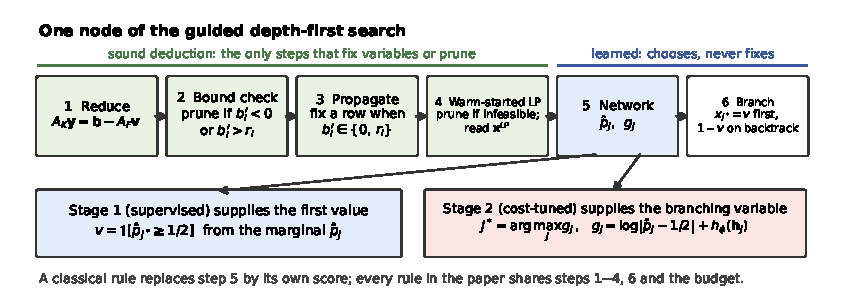
\includegraphics[width=\textwidth]{framework.pdf}
\caption{The guided depth-first search. Inside a node, steps 1--4 are sound and are the only steps that fix variables or prune; the network at step 5 only chooses, the value from Stage~1 and the variable from Stage~2. Lattice reduction, when used, runs before the search as a preprocessing step and is switched off in every branching comparison.}
\label{fig:framework}
\end{figure*}

\section{Related work}
\label{sec:related}

\paragraph{Marginals of the solution set as a branching signal.} Branching on the fraction of solutions that agree with a decision predates learning: counting-based search \citep{pesant2012counting} branches on the variable--value pair of maximum solution density computed inside individual constraints, and belief-propagation-guided decimation \citep{montanari2007solving} fixes the most biased variable under approximate marginals. NSNet \citep{li2022nsnet} trains a graph network on exact marginals of the satisfying assignments of a SAT formula, obtained by enumerating them, and rounds the estimates into an initial assignment for local search; MIP-GNN \citep{khalil2022mipgnn}, Neural Diving \citep{nair2020solving} and predict-and-search \citep{han2023gnn} predict per-variable biases from collected near-optimal solutions and use them to fix variables, warm-start or restrict a search. Stage~1 shares NSNet's target and differs in where and how it is used: the marginals are conditional and carried to every node of a complete search by the reduction identity, they guide branching without fixing anything, and the $\FORCED$/$\FREE$ partition and the controlled in-tree-versus-root comparison have no counterpart in that work.

\paragraph{Learning to branch.} \citet{khalil2016learning} and \citet{gasse2019exact} imitate strong branching, the latter with the bipartite variable--constraint graph network we also use; imitation targets an expert's ranking rather than the tree size the ranking is meant to reduce. Optimising tree size directly is the subject of a line of reinforcement-learning work: FMSTS \citep{etheve2020reinforcement} uses the size of a node's subtree as an observable Q-value, shows that under depth-first search minimising every subtree minimises the whole tree, and learns from scratch; tree MDPs \citep{scavuzzo2022learning} formalise the per-subtree credit assignment; retro branching \citep{parsonson2023reinforcement} learns from retrospectively extracted subtree trajectories; SORREL \citep{sorrel2025} initialises from demonstrations. Neuro\# \citep{vaezipoor2021learning} trains a graph network on the residual formula of a \#SAT solver by evolution strategies and generalises to larger instances. Stage~2 uses the FMSTS credit assignment with a plain policy gradient \citep{williams1992simple}; what it adds is the starting point and the scope, a rule derived from exact marginals, frozen, with only the branching order learned. The classical statements of the objective are the fail-first principle \citep{haralick1980increasing} and impact-based search \citep{refalo2004impact}. Value ordering has been learned in constraint programming from solutions \citep{chu2015learning} and by deep Q-learning \citep{cappart2021combining}; we take the value from the exact posterior and learn only the variable.

\paragraph{Market split, lattice methods and complete solvers.} The market split problem of \citet{cornuejols1999class} is the benchmark that exposes the weakness of branch-and-bound on systems like~\eqref{eq:bls}: $m$ equality rows over $n=10(m-1)$ binary variables, coefficients drawn uniformly from $\{0,\dots,99\}$, and each right-hand side set to half its row sum, so that the relaxation polytope is wide, its vertices far from integrality, and bounding prunes almost nothing; branch-and-cut stops at $m\approx7$. \citet{aardal2000diophantine,aardal2000market} solved these instances by reformulating them on a lattice: the Aardal--Hurkens--Lenstra embedding turns a solution into one of the shortest vectors of a lattice, LLL/BKZ reduction \citep{lenstra1982factoring,schnorr1994lattice} finds it, and the recovered vector is verified, so the method is sound. Lattice enumeration remains the state of the art on the benchmark: \citet{wassermann2025solving} solves QOBLIB market-split instances up to $m=14$ on one CPU. Our instances share the ingredients that make market split hard, dense rows and right-hand sides at the middle of their range, and differ in having $0/1$ coefficients, a planted solution and a search regime of up to $80$ variables; lattice reduction is therefore the natural first stage of a BLS solver, and our contribution begins where it stops working. Constraint solvers with clause learning \citep{marquessilva1999grasp,ohrimenko2009propagation} manufacture information as they descend and set the wall-clock reference we compare against. Direct satisfiability prediction has a weak record \citep{selsam2019neurosat,li2023g4satbench}, and message-passing networks provably cannot separate some feasible/infeasible pairs \citep{chen2023representing}. Both learned stages of our method are instances of amortised inference \citep{amos2023tutorial,gershman2014amortized}: the marginal network replaces one relaxation per variable, the cost head replaces a completed search.

\paragraph{What these approaches leave open for a BLS.} The three learned-branching families closest to our setting each lose something essential when transplanted to a feasibility system, and Section~\ref{sec:exp} runs each transplant inside the same search loop as our rule.
\emph{Imitation of strong branching} \citep{khalil2016learning,gasse2019exact} presupposes an objective: the expert scores a candidate by the bound improvement of its two children, and a BLS has no bound to improve. The only information strong branching retains on a feasibility system is whether a child's relaxation is infeasible, so the expert degenerates to LP probing, a rule that fixes what it can refute and then branches on the LP value. We run that expert directly (Section~\ref{sec:rq1}); it expands the fewest nodes of any unlearned rule and pays one relaxation per free variable per node, which costs it $5$--$6\times$ the wall-clock of the learned rule. Imitating it would inherit its ranking without its cost, and the ranking is not the one that minimises the tree (Section~\ref{sec:rq3}).
\emph{Approximate marginals by message passing} \citep{li2022nsnet,montanari2007solving} are well defined for a BLS: each row is a cardinality factor, and sum-product with exact factor messages is implementable. Two things go wrong. The factor graph is dense, every row touching about a third of the variables, so loopy belief propagation needs heavy damping and hundreds of iterations where it converges; and NSNet-style use estimates marginals once at the root and decodes an assignment for an incomplete local search, whereas a complete search needs marginals \emph{conditional} on the partial assignment at every node. We run damped sum-product in the Stage-1 slot: its trees are the size of Stage~1's, and one estimate costs about $30\times$ a network forward pass (Section~\ref{sec:rq1}). The learned marginal network is, in this sense, amortised belief propagation.
\emph{Reinforcement learning from scratch on subtree size} \citep{etheve2020reinforcement,scavuzzo2022learning} supplies the right credit assignment, and we keep it. What it does not supply is the value choice: a single policy over variable--value pairs must learn which value to try first from the same sparse reward that teaches it which variable to branch on, while a BLS makes the optimal value available exactly, as a conditional marginal, on the instances it can be enumerated on. Section~\ref{sec:rq3} separates the two signals with a value-by-variable cross ablation and starts the cost-tuned policy from a random head, from the LP rule and from the marginal rule; it also reports a result that cuts against our own design, namely that once the variable choice is learned, the LP rounding value does as well as the exact-marginal value.
Two further gaps are not about learning. Lattice reduction with bounded enumeration \citep{aardal2000market,wassermann2025solving} is sound and solves every instance we study, in a fraction of a second at $n=60$ and in minutes at $n=80$, where it is slower than the learned search (Section~\ref{sec:rq4}); it is a natural preprocessing step for a BLS solver, and the comparison of branching rules in this paper is made on the search alone, with the lattice stage switched off. And a network cannot be trusted with a verdict on feasibility \citep{selsam2019neurosat,chen2023representing}, so none of our stages is asked for one: the marginal and the cost head only order the search, and the search stays complete.

\section{Problem statement and preliminaries}
\label{sec:problem}

\subsection{Instances and scope}
\label{sec:problem-instances}

We study feasible instances of~\eqref{eq:bls}: every instance is generated by planting a solution, so $\SOL\neq\emptyset$, and deciding infeasibility is outside the scope of this paper. The construction is the market-split recipe of Section~\ref{sec:related} with $0/1$ coefficients. The generator draws a random $A$ in which each entry is $1$ with probability $p$, plants a random $\mathbf{x}^\ast$ with exactly $n/2$ ones and sets $\mathbf{b}=A\mathbf{x}^\ast$, so every right-hand side sits at the middle of its row's range, where the number of $0/1$ completions is largest and propagation cannot fire. Among $20$ candidate plantings per $A$ it keeps the one whose relaxation polytope is widest, measured by the mean distance between the vertices returned by four random linear objectives; the relaxation of the kept instance is therefore as uninformative as the generator can make it. Uniqueness is not imposed; the median number of solutions, where enumeration completes, is $64$, $112$ and $113$ at $n=25$, $50$ and $60$. Every result in this paper is at one density, $p=0.3$. The density is not fixed by the application, and Section~\ref{sec:exp-setup} reports the sweep over $p\in\{0.2,0.3,0.4,0.5\}$ that led to this choice; at $p=0.5$, the density of the market-split benchmark, the learned rule and the best classical rule are indistinguishable, and we say so there.

\subsection{Conditioning is reduction}
\label{sec:problem-reduce}

\begin{figure*}[t]
\centering
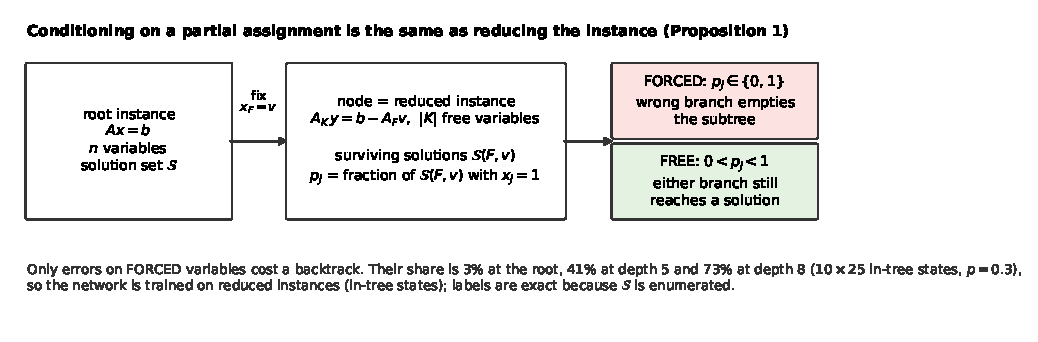
\includegraphics[width=\textwidth]{reduction.pdf}
\caption{Proposition~\ref{prop:reduce} and the partition it induces. A node with $\mathbf{x}_F=\mathbf{v}$ is the smaller BLS $A_K\mathbf{y}=\mathbf{b}-A_F\mathbf{v}$; its conditional marginals are the ordinary marginals of that instance. Variables on which every surviving solution agrees are $\FORCED$; only branching against them costs a backtrack.}
\label{fig:reduction}
\end{figure*}

A node of a depth-first search over~\eqref{eq:bls} is a partial assignment $\mathbf{x}_F=\mathbf{v}$ on a set $F$ of fixed variables, with $K$ the free ones. Let $\SOL(F,\mathbf{v})=\{\mathbf{x}\in\SOL:\mathbf{x}_F=\mathbf{v}\}$ be the solutions consistent with the node and
\begin{equation}
p_j=\Pr[x_j{=}1\mid A,\mathbf{b},\mathbf{x}_F{=}\mathbf{v}]=\frac{|\{\mathbf{x}\in\SOL(F,\mathbf{v}):x_j{=}1\}|}{|\SOL(F,\mathbf{v})|},\quad j\in K,
\label{eq:marginal}
\end{equation}
the conditional marginal, defined by the uniform measure on $\SOL$ (the planted generator does not induce this measure; it is the definition of the target).

\begin{proposition}
\label{prop:reduce}
With $A_F,A_K$ the column submatrices indexed by $F,K$, the map $\mathbf{x}\mapsto\mathbf{x}_K$ is a bijection from $\SOL(F,\mathbf{v})$ onto $\{\mathbf{y}\in\{0,1\}^{|K|}:A_K\mathbf{y}=\mathbf{b}-A_F\mathbf{v}\}$. Hence the conditional marginals of the original instance are the ordinary marginals of the reduced instance.
\end{proposition}
\begin{proof}
$A\mathbf{x}=A_F\mathbf{x}_F+A_K\mathbf{x}_K$; with $\mathbf{x}_F=\mathbf{v}$ fixed, $A\mathbf{x}=\mathbf{b}$ iff $A_K\mathbf{x}_K=\mathbf{b}-A_F\mathbf{v}$, and $\mathbf{x}_F$ is determined, so the map is a bijection; the marginal statement follows by counting.
\end{proof}

Two consequences (Figure~\ref{fig:reduction}). First, one architecture, one label generator and one training loop serve every node: a depth-$d$ training state is stored as an instance on $n-d$ variables, and a network trained on small instances is evaluated on the reduced instances that a search on a larger one produces. Second, $p_j\in\{0,1\}$ means every surviving solution agrees on $x_j$, and branching the other way empties the subtree. We call such variables $\FORCED$ and the rest $\FREE$: either branch of a $\FREE$ variable still reaches a solution, so a wrong first value costs nothing beyond exploring a subtree that contains one. Only $\FORCED$ errors cost a backtrack.

\subsection{What a node looks like, and the accuracy ceiling}
\label{sec:problem-ceiling}

Because $\SOL(F,\mathbf{v})$ can be enumerated on small instances, the Bayes-optimal per-variable accuracy of any predictor of a solution is computable,
\begin{equation}
\mathrm{ceil}(F,\mathbf{v})=\frac{1}{|K|}\sum_{j\in K}\max(p_j,1-p_j),
\label{eq:ceiling}
\end{equation}
attained by answering the majority value of the surviving solutions. On held-out in-tree states of $10\times25$ instances at $p=0.3$ the surviving solution set shrinks from a median of $74$ at the root to a singleton by depth $10$, and the $\FORCED$ share of the free variables rises from $3\%$ at the root to $41\%$ at depth $5$, $73\%$ at depth $8$ and $94\%$ at depth $12$. At the root almost no decision can cost anything and the ceiling~\eqref{eq:ceiling} is dominated by $\FREE$ variables; from depth $6$ on, most decisions can. Figure~\ref{fig:prediction} shows the Stage-1 network against that ceiling by depth. This is the regime a branching heuristic must be good in, and it is where prediction is trained and evaluated below.


\begin{figure}[t]
\centering
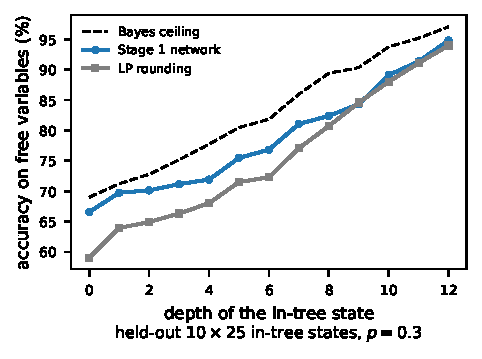
\includegraphics[width=\columnwidth]{prediction.pdf}
\caption{Prediction against the exact marginals on held-out in-tree states of $10\times25$ instances at $p=0.3$, by depth: per-variable accuracy of the Stage-1 network and of relaxation rounding against the Bayes ceiling~\eqref{eq:ceiling}.}
\label{fig:prediction}
\end{figure}

\section{Proposed method}
\label{sec:method}

\subsection{Overview}
\label{sec:method-overview}

The solver is a depth-first search whose branching decisions are guided by a learned network (Figure~\ref{fig:framework}); nothing learned ever fixes a variable or prunes, so the search stays complete. The network (Figure~\ref{fig:network}) is trained in two stages (Figure~\ref{fig:training}): Stage~1 fits its marginal head to exact conditional marginals of enumerated instances, Stage~2 adds a policy head on the frozen trunk and fine-tunes it on the exact number of nodes that every branching decision costs. Lattice reduction in the Aardal--Hurkens--Lenstra embedding \citep{aardal2000diophantine}, with bounded enumeration after BKZ, is a sound preprocessing step that solves every instance we study, cheaply at small sizes (Section~\ref{sec:rq4}); it is not part of the method and is switched off in every comparison of branching rules, so that the measured difference is the branching decision and nothing else.

\subsection{Guided depth-first search}
\label{sec:method-search}

Every instance is searched from scratch by the depth-first procedure of Algorithm~\ref{alg:node}. A node is a partial assignment; by Proposition~\ref{prop:reduce} it is handled as the reduced instance $(A',\mathbf{b}')=(A_K,\mathbf{b}-A_F\mathbf{v})$, and $r_i$ denotes the number of free variables in row $i$ of $A'$.

\begin{table}[t]
\centering
\caption{Algorithm 1: one node of the guided depth-first search. Steps 1--4 are sound and are the only steps that fix variables or prune; the learned components enter only at step 5.}
\label{alg:node}
\fitc{\begin{tabular}{@{}rp{0.9\columnwidth}@{}}
\toprule
1 & \textbf{Reduce.} Pop $(F,\mathbf{v})$; form $A'=A_K$, $\mathbf{b}'=\mathbf{b}-A_F\mathbf{v}$. Drop rows with $r_i=0$; if none remain, verify $A\mathbf{x}=\mathbf{b}$ and return $\mathbf{x}$. \\
2 & \textbf{Bound check.} If $b'_i<0$ or $b'_i>r_i$ for some row, discard the node. \\
3 & \textbf{Propagate.} While some row has $b'_i=0$ (fix its free variables to $0$) or $b'_i=r_i$ (fix them to $1$): apply the fixings; on a contradiction discard the node; if variables were fixed, push the reduced node and return. \\
4 & \textbf{Relax.} Re-optimise the single warm-started relaxation $\{A\mathbf{x}=\mathbf{b},\ 0\le\mathbf{x}\le1\}$ with the bounds of $F$ tightened to $\mathbf{v}$ (dual simplex from the previous basis, $0.08$\,ms). If infeasible, discard the node; else read the vertex $\mathbf{x}^{LP}_K$. \\
5 & \textbf{Predict.} One forward pass of the network on the bipartite graph of $(A',\mathbf{b}',\mathbf{x}^{LP}_K)$ gives $\hat p_j$ and $g_j$ for $j\in K$ ($0.3$--$0.5$\,ms on the dense path of Section~\ref{sec:method-cost}). Choose $j^\star=\arg\max_j g_j$ and $v=\mathbb{1}[\hat p_{j^\star}\ge\frac12]$. \\
6 & \textbf{Branch.} Push the child $x_{j^\star}=1-v$, then the child $x_{j^\star}=v$, so that $v$ is explored first and $1-v$ on backtracking. \\
\bottomrule
\end{tabular}}
\end{table}

Three design choices matter for what follows. Propagation on a $0/1$ row reads ``exactly $b'_i$ of the $r_i$ free variables in this row are $1$'' and can fix variables only when $b'_i\in\{0,r_i\}$, which is why it is inert near the root of our instances. The relaxation is not rebuilt per node: one linear program over the original $n$ variables is kept for the whole search and a node is expressed as a set of bound changes, so consecutive nodes, a child or a sibling after backtracking, differ by a few bounds and the dual simplex resumes from the parent basis; this is $50\times$ cheaper than rebuilding and is what lets the loop process about $1{,}000$ nodes per second in Python. Its infeasibility test is strictly stronger than propagation, since it sees linear combinations of rows, and it is the last sound step before the network. The vertex $\mathbf{x}^{LP}$ it returns is the main input feature of the network.

\subsection{Stage 1: exact conditional marginals as the target}
\label{sec:method-stage1}

\begin{figure*}[t]
\centering
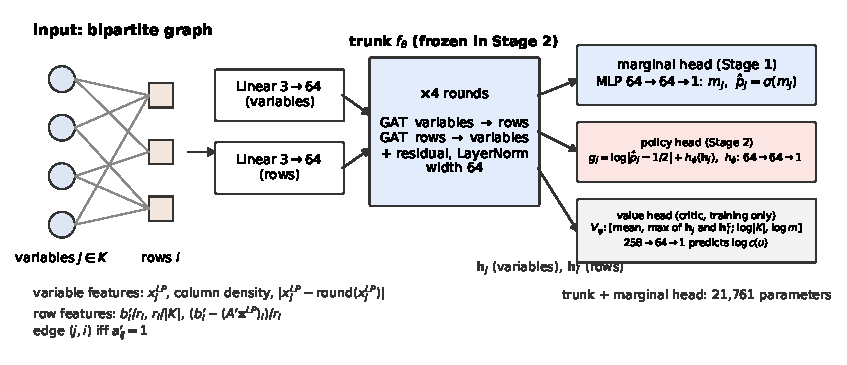
\includegraphics[width=\textwidth]{network.pdf}
\caption{The network. The reduced instance enters as a bipartite graph with three features per variable and per row; a trunk of four graph-attention rounds produces an embedding per variable and per row; three heads read them. The marginal head is trained in Stage~1, the policy head in Stage~2 on the frozen trunk, and the value head serves only as the critic during Stage~2.}
\label{fig:network}
\end{figure*}

\begin{figure*}[t]
\centering
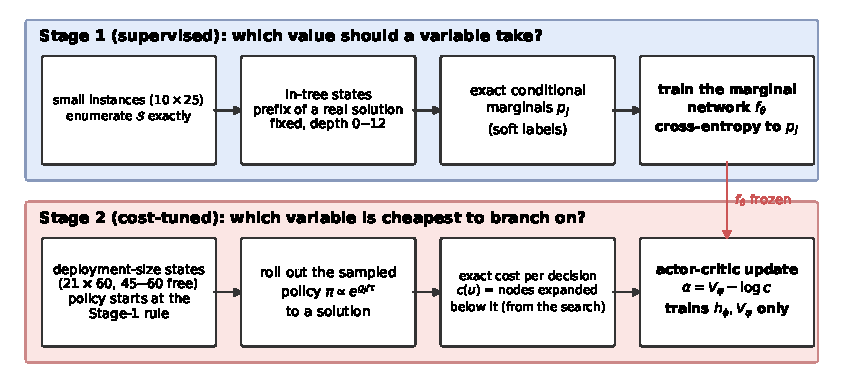
\includegraphics[width=\textwidth]{training.pdf}
\caption{The two training stages. Stage~1 learns \emph{which value} from exact conditional marginals of enumerable instances; Stage~2 learns \emph{which variable} from the exact number of nodes every decision costs, produced by the search, with the Stage-1 network frozen.}
\label{fig:training}
\end{figure*}

\paragraph{Network.} The network $f_\theta$ (Figure~\ref{fig:network}) is a bipartite variable--constraint graph network with graph attention \citep{velickovic2018graph}, the architecture family of \citet{gasse2019exact}. Each variable node carries three features (its relaxation value $x^{LP}_j$, its column density, its fractionality $|x^{LP}_j-\mathrm{round}(x^{LP}_j)|$), each constraint node three (its right-hand side $b'_i/r_i$, its density $r_i/|K|$, its relaxation residual $(b'_i-(A'\mathbf{x}^{LP})_i)/r_i$), and an edge joins $j$ to $i$ where $a'_{ij}=1$. Linear layers lift both to width $64$; four rounds of attention then alternate variable-to-constraint and constraint-to-variable messages with residual connections and layer normalisation, and a two-layer marginal head maps each variable embedding $\mathbf{h}_j$ to one logit, $\hat p_j=\sigma(m_j)$; $21{,}761$ parameters in all. The two heads added in Stage~2 are described in Section~\ref{sec:method-stage2}. The architecture is standard; the contribution is the target.

\paragraph{Target and training states.} On instances small enough to enumerate ($10\times25$), $\SOL$ is obtained with the all-solutions mode of a constraint solver and $p_j$ computed by counting. Only enumerations that run to exhaustion are accepted; a time-limited enumeration with solutions already collected would substitute a truncated $\SOL$ and bias every label. Training states are reachable in-tree states: a depth $d\in\{0,\dots,12\}$ is drawn uniformly, a prefix of an LP-confidence variable ordering is fixed to the values of a randomly chosen actual solution, and the reduced instance is enumerated in turn to give $p_j$ on its free variables. The network is trained by cross-entropy against the soft targets,
\begin{equation}
\mathcal{L}_1=-\tfrac{1}{|K|}\sum_{j\in K}\bigl[p_j\log\hat p_j+(1-p_j)\log(1-\hat p_j)\bigr],
\label{eq:loss1}
\end{equation}
which is minimised exactly at $\hat p=p$; replacing $p_j$ by the planted solution, the usual choice, is a noisy surrogate whenever $|\SOL|>1$.

\paragraph{Branching rule.} At a node the network is evaluated once and the Stage-1 rule branches on the most confident marginal with its majority value,
\begin{equation}
j^\star=\arg\max_{j\in K}\,|\hat p_j-\tfrac12|,\qquad v=\mathbb{1}[\hat p_{j^\star}\ge\tfrac12].
\label{eq:rule1}
\end{equation}

\subsection{Stage 2: exact subtree node counts as the objective}
\label{sec:method-stage2}

Rule~\eqref{eq:rule1} tries first the value that the larger share of surviving solutions takes, so that the first child keeps as many solutions as the marginal can promise. It says nothing about how much the search pays when it does not, nor how much smaller the children become; both are properties of the subtree, and a depth-first search produces them exactly. For a node $u$ let $c(u)$ be the number of nodes expanded below $u$ until a solution is found there or the subtree is exhausted; the search returns it when it backtracks out of $u$. We use $c(u)$ as the cost of the branching decision made at $u$; $c(\text{root})$ is the number of nodes the whole search expands to reach a solution, which is the tree-size metric reported throughout the experiments. Stage~2 fine-tunes the branching order on $-\log c(u)$.

\paragraph{Decision process.} A state is the reduced instance after propagation; an action is a free variable $j$; the first value stays $\mathbb{1}[\hat p_j\ge\frac12]$ from the frozen Stage-1 network. Because each decision owns its subtree, credit is assigned per decision rather than per episode, the property a sparse solved/unsolved reward lacks and the one that makes the problem well posed \citep{etheve2020reinforcement}.

\paragraph{Policy and value heads.} On the frozen trunk of $f_\theta$ two heads are added (Figure~\ref{fig:network}). The policy logit is
\begin{equation}
g_j(s)=\log\bigl|\hat p_j-\tfrac12\bigr|+h_\phi(\mathbf{h}_j),
\label{eq:policy}
\end{equation}
with $h_\phi$ a two-layer network whose last layer is initialised to zero, so that $\pi(j\mid s)\propto\exp(g_j/\tau)$ starts as a softening of rule~\eqref{eq:rule1} and its argmax is exactly that rule. A value head $V_\psi(s)$ on the mean- and max-pooled variable and constraint embeddings, $\log|K|$ and $\log m$ predicts $\log c$.

\paragraph{Update.} Each epoch samples $400$ training states with $45$--$60$ free variables, rolls the sampled policy ($\tau=1$) out to a solution, and records every decision with its exact cost, about $21{,}000$ decisions per epoch. With the advantage $\alpha(u)=V_\psi(s_u)-\log c(u)$ standardised within the epoch,
\begin{equation}
\begin{split}
\mathcal{L}_2=\sum_u\Bigl[&-\alpha(u)\log\pi(j_u\mid s_u)-\lambda\,\mathcal{H}\bigl(\pi(\cdot\mid s_u)\bigr)\\
&+\bigl(V_\psi(s_u)-\log c(u)\bigr)^2\Bigr],\qquad\lambda=0.01,
\end{split}
\label{eq:loss2}
\end{equation}
an on-policy actor-critic update with Monte-Carlo returns \citep{williams1992simple}; no bootstrapping is needed because the return is exact. Only $\phi,\psi$ are trained; $\theta$ is fixed, so the marginal that chooses values and defines the $\FORCED$/$\FREE$ partition is unchanged, and any improvement is attributable to the branching order alone. The critic is pre-trained on decisions recorded under rule~\eqref{eq:rule1}, and its held-out rank correlation with $\log c$ gates the actor update, since a baseline that cannot rank costs turns the advantage into noise. The epoch is selected by the total node count below held-out states of the training pool, never on evaluation instances. At deployment the policy is greedy, $j^\star=\arg\max_j g_j(s)$.

\subsection{Cost per node}
\label{sec:method-cost}

At a node with $|K|$ free variables the guided search pays one warm-started relaxation and one forward pass. The forward pass runs on a dense adjacency tensor through TorchScript (the graphs have at most $80$ variables and $28$ rows, so sparse message passing buys nothing), single-threaded, in $0.3$--$0.5$\,ms depending on the number of free variables; the Stage-2 heads add nothing measurable. A single-relaxation classical rule pays the relaxation alone, so the learned rule's node is $1.3$--$1.5\times$ as expensive, with the ratio falling as the relaxation grows with size (Section~\ref{sec:rq1}, Table~\ref{tab:profile}). The sound procedure that detects the same $\FORCED$ variables, LP probing (fix $x_j$ to each value and prune the one that makes the relaxation infeasible), pays $|K|$ relaxations per node.

\section{Experiments}
\label{sec:exp}

The experiments answer the four questions of Section~\ref{sec:intro} in turn (Sections~\ref{sec:rq1}--\ref{sec:rq4}), after the setup. Every number in this section comes from instances of one density, $p=0.3$; nothing is pooled across densities.

\subsection{Setup}
\label{sec:exp-setup}

\paragraph{Instances.} Instances are generated as in Section~\ref{sec:problem-instances}. Sizes are $10\times25$, $18\times50$, $21\times60$, $24\times70$ and $28\times80$ with constraint density $m/n\approx0.35$ throughout; the evaluation sets hold $30$ instances at the two smallest sizes and $100$ at each of the three largest, all disjoint from the training pools by generator seed. Stage~1 trains on in-tree states of $1{,}600$ separate $10\times25$ instances, Stage~2 on states of $500$ separate $21\times60$ instances. At $n=100$ no method, learned or not, solves an instance within $20$\,s of CP-SAT, so $n=80$ is the last size.

\paragraph{Why one density, and why $0.3$.} The density of $A$ is not fixed by the application, and the market-split benchmark uses $p=\frac12$. Table~\ref{tab:density} reports the sweep that decided the question: at each of four densities we generated evaluation sets, ran the single-relaxation classical rules of Table~\ref{tab:arms} and the learned rule, and recorded the node ratio between the strongest classical rule and the learned rule. At $p=0.2$ the instances are easy and every rule's tree is close to the propagation floor; at $p=0.5$ the learned rule and most-fractional branching are indistinguishable; the gap is largest at $p=0.3$ and $p=0.4$. We fixed $p=0.3$ before running anything in Sections~\ref{sec:rq1}--\ref{sec:rq4}, retrained both stages on $p=0.3$ data, and report nothing from the other densities beyond this table. The choice is favourable to the method and is stated as such: the claims of this paper are claims about this density.

\begin{table}[t]
\centering
\caption{Density sweep that fixed $p=0.3$: at each density and size, the strongest single-relaxation classical rule (by median nodes) against the learned rule, median per-instance node ratio with $95\%$ bootstrap interval and sign-test $p$-value. The learned rule was trained at $p=0.5$ for the $p=0.5$ rows and at $p=0.3$ for all others. Sets of $30$ instances are marked; the rest have $100$.}
\label{tab:density}
\footnotesize
\fitc{\begin{tabular}{llrlrrlr}
\toprule
$p$ & size & $n$ & strongest classical & its nodes & Stage 1+2 nodes & ratio [CI] & $p$-value \\
\midrule
0.2 & $21\times60$ & 100 & dom/wdeg & 40 & 39 & 1.03$\times$ [0.89, 1.14] & $0.84$ \\
0.2 & $24\times70$ & 30 & dom/wdeg & 112 & 64 & 1.75$\times$ [1.03, 2.45] & $0.10$ \\
\addlinespace
0.3 & $21\times60$ & 100 & dom/wdeg & 436 & 325 & 1.52$\times$ [1.08, 1.95] & $0.04$ \\
0.3 & $24\times70$ & 100 & dom/wdeg & 5,263 & 2,580 & 1.79$\times$ [1.15, 2.42] & $0.04$ \\
0.3 & $28\times80$ & 100 & maxSD & 141,178 & 58,026 & 3.20$\times$ [2.29, 4.79] & $10^{-9}$ \\
\addlinespace
0.4 & $21\times60$ & 100 & dom/wdeg & 4,265 & 1,711 & 2.34$\times$ [1.82, 3.35] & $4\cdot10^{-4}$ \\
0.4 & $24\times70$ & 100 & maxSD & 55,018 & 24,843 & 2.05$\times$ [1.33, 2.82] & $7\cdot10^{-3}$ \\
0.4 & $28\times80$ & 100 & maxSD & 578,231 & 327,660 & 2.20$\times$ [1.41, 3.06] & $10^{-5}$ \\
\addlinespace
0.5 & $21\times60$ & 100 & most-fractional & 6,010 & 5,495 & 1.28$\times$ [0.92, 1.94] & $0.13$ \\
0.5 & $24\times70$ & 30 & most-fractional & 64,232 & 90,054 & 0.66$\times$ [0.34, 2.01] & $0.86$ \\
0.5 & $28\times80$ & 30 & maxSD & 402,570 & 281,760 & 1.76$\times$ [1.03, 4.15] & $0.04$ \\
\bottomrule
\end{tabular}}
\end{table}

\paragraph{Training.} Stage~1: $1{,}600$ instances of $10\times25$ enumerated to exhaustion, eight in-tree states per instance at depths $0$--$12$, $10{,}000$ training and $2{,}000$ test states; Adam, learning rate $10^{-3}$, $20$ epochs, batch $1$, gradient clipping $1.0$, about $20$ minutes on one CPU core, no hyperparameter tuned and no validation split. Its accuracy on $\FORCED$ variables of the test states is $79.1\%$ against a Bayes ceiling of $83.3\%$ and $76.0$--$77.5\%$ for relaxation rounding. Stage~2: critic pre-training on decisions recorded under the Stage-1 rule on $21\times60$ states with $45$--$60$ free variables (held-out Spearman correlation with $\log c$ of $0.81$, against $0.75$ for a baseline that knows only the state's size), then six epochs of the update~\eqref{eq:loss2}; the epoch is selected on held-out training states (epoch $6$, at $0.36$ of the Stage-1 rule's node count below those states).

\begin{table*}[t]
\centering
\caption{Branching rules compared. All run in the same depth-first loop (Algorithm~\ref{alg:node}: one warm-started relaxation per node, the same propagation, the same budget) and differ only in step 5. The single-relaxation classical rules cost one relaxation per node; LP probing costs one per free variable; the reference signals are not deployable and bound what a value signal can do.}
\label{tab:arms}
\small\begin{tabular}{llll}
\toprule
group & rule & branches on & first value \\
\midrule
classical & LP rule (most-integral) & $\arg\max_j|x^{LP}_j-\tfrac12|$ & $\mathrm{round}(x^{LP}_j)$ \\
& most-fractional & $\arg\min_j|x^{LP}_j-\tfrac12|$ & $\mathrm{round}(x^{LP}_j)$ \\
& maxSD \citep{pesant2012counting} & max.\ solution density of a row & the dense value \\
& dom/wdeg \citep{boussemart2004boosting} & max.\ weighted failure degree & $\mathrm{round}(x^{LP}_j)$ \\
& impact \citep{refalo2004impact} & max.\ averaged search-space reduction & the smaller-impact value \\
& LP probing (= strong branching on a BLS) & fixes refutable values, then LP rule & $\mathrm{round}(x^{LP}_j)$ \\
& uniform & a uniformly random free variable & uniform \\
\midrule
reference & oracle marginals & $\arg\max_j|p_j-\tfrac12|$, $p_j$ exact by enumeration & $\mathbb{1}[p_j\ge\tfrac12]$ \\
& BP marginals (NSNet-based) & as above with damped sum-product $\tilde p_j$ & $\mathbb{1}[\tilde p_j\ge\tfrac12]$ \\
\midrule
learned & Stage 1 & most confident marginal, $\arg\max_j|\hat p_j-\tfrac12|$ & $\mathbb{1}[\hat p_j\ge\tfrac12]$ \\
& Stage 1+2 & cost-tuned score, $\arg\max_j g_j$ & $\mathbb{1}[\hat p_j\ge\tfrac12]$ \\
\bottomrule
\end{tabular}
\end{table*}

\paragraph{Rules.} Table~\ref{tab:arms} lists the rules. The two LP rules are the most-integral and most-fractional vertex rules; maxSD is counting-based search, whose solution density on a $0/1$ row is exactly $b'_i/r_i$ and therefore costs nothing to compute; dom/wdeg and impact are the two standard adaptive rules of constraint programming, implemented with the failure and reduction statistics of our own loop; LP probing is what strong branching reduces to without an objective; the uniform rule checks that the instances are hard. The oracle enumerates $\SOL(F,\mathbf{v})$ at every node and is run where that is affordable; the BP rule runs sum-product with exact cardinality-factor messages, damping $0.9$ and up to $300$ iterations. The learned baselines of Section~\ref{sec:related} appear as follows: LP probing stands for imitation of strong branching (it is the expert itself), BP for message-passing marginals, and in Section~\ref{sec:rq3} cost-tuned policies started from a random head and from the LP rule stand for reinforcement learning from scratch and from a classical rule.

\paragraph{Protocol and statistics.} Two metrics are recorded per instance: the number of nodes expanded to reach a solution, $c(\text{root})$ of Section~\ref{sec:method-stage2}, which measures branching quality and is seed-invariant because the search is deterministic given the relaxation vertex; and single-threaded wall-clock time, which also reflects the cost per node. Budgets are $60$, $300$, $600$, $1{,}200$ and $1{,}200$\,s per instance for the five sizes, enforced by process termination; six instances run concurrently on a $20$-core machine, no GPU is used, and the learned arms use the dense TorchScript path of Section~\ref{sec:method-cost}. Comparisons are paired by instance: we report the median of the per-instance ratios on the instances both rules solved, a $95\%$ bootstrap interval of that median ($1{,}000$ resamples of instances), the number of instances on which each rule wins, and a two-sided exact sign test with ties excluded; PAR-2 (mean time with an unsolved instance counted at twice the budget) summarises solve rate and time together. Medians of raw node and time values are given for orientation and are not what the tests act on. The timing of the learned arms is replicated over two further evaluation seeds in Appendix~\ref{app:seeds}.

\subsection{RQ1: against classical branching and transplanted learned branching}
\label{sec:rq1}

\begin{table*}[t]
\centering
\caption{Branching rules in the same search loop at $p=0.3$, $100$ instances per size. Medians are over solved instances; the last two columns are the median per-instance ratio of the rule to Stage~1+2 on commonly solved instances, its $95\%$ bootstrap interval, and the two-sided sign test $p$-value (ties excluded). A ratio above $1$ means the rule expands more nodes or takes longer than the learned rule. PAR-2 counts an unsolved instance at twice the budget.}
\label{tab:rq1}
\footnotesize
\begin{tabular}{lrrrrll}
\toprule
rule & solved & med.\ nodes & med.\ s & PAR-2 s & nodes, rule / Stage 1+2 & time, rule / Stage 1+2 \\
\midrule
\multicolumn{7}{l}{\emph{21$\times$60 (100), budget 600\,s}} \\
LP rule (most-integral) & 100/100 & 7,762 & 4.58 & 8.0 & 23.90$\times$ [15.11, 37.29] $10^{-25}$ & 10.55$\times$ [7.68, 18.48] $10^{-22}$ \\
most-fractional & 100/100 & 662 & 0.41 & 0.7 & 2.27$\times$ [1.29, 4.39] $10^{-4}$ & 1.13$\times$ [0.79, 1.57] $0.48$ \\
maxSD & 100/100 & 494 & 0.30 & 0.7 & 1.52$\times$ [1.13, 2.45] $10^{-3}$ & 0.77$\times$ [0.61, 1.32] $0.48$ \\
dom/wdeg & 100/100 & 436 & 0.25 & 0.5 & 1.52$\times$ [1.08, 1.95] $0.04$ & 0.83$\times$ [0.61, 0.96] $0.02$ \\
impact & 100/100 & 1,464 & 2.68 & 5.8 & 5.76$\times$ [2.69, 7.72] $4\cdot10^{-9}$ & 7.06$\times$ [3.98, 12.84] $10^{-15}$ \\
LP probing & 100/100 & 130 & 1.99 & 2.9 & 0.37$\times$ [0.28, 0.44] $10^{-6}$ & 5.36$\times$ [4.47, 6.32] $10^{-22}$ \\
uniform & 100/100 & 2,112 & 1.21 & 2.0 & 5.12$\times$ [3.66, 9.31] $10^{-14}$ & 2.81$\times$ [1.98, 4.26] $10^{-10}$ \\
Stage 1 & 100/100 & 628 & 0.65 & 1.2 & 2.32$\times$ [1.08, 3.25] $0.01$ & 2.02$\times$ [1.19, 2.83] $10^{-3}$ \\
\textbf{Stage 1+2} & 100/100 & \textbf{325} & \textbf{0.36} & 0.6 & --- & --- \\
\midrule
\multicolumn{7}{l}{\emph{24$\times$70 (100), budget 1200\,s}} \\
LP rule (most-integral) & 100/100 & 95,440 & 51.95 & 81.5 & 37.74$\times$ [27.17, 66.01] $8\cdot10^{-27}$ & 21.88$\times$ [16.38, 40.52] $8\cdot10^{-27}$ \\
most-fractional & 100/100 & 6,504 & 3.97 & 6.8 & 3.67$\times$ [2.13, 4.69] $6\cdot10^{-11}$ & 2.43$\times$ [1.42, 2.94] $4\cdot10^{-4}$ \\
maxSD & 100/100 & 5,637 & 3.23 & 5.4 & 2.46$\times$ [1.71, 3.10] $10^{-7}$ & 1.46$\times$ [1.10, 1.87] $4\cdot10^{-3}$ \\
dom/wdeg & 100/100 & 5,263 & 2.73 & 3.9 & 1.79$\times$ [1.15, 2.42] $0.04$ & 1.09$\times$ [0.68, 1.37] $0.48$ \\
impact & 100/100 & 16,256 & 33.07 & 64.7 & 8.92$\times$ [5.57, 10.95] $8\cdot10^{-14}$ & 19.01$\times$ [12.89, 25.36] $6\cdot10^{-24}$ \\
LP probing & 100/100 & 1,088 & 14.27 & 23.4 & 0.36$\times$ [0.24, 0.57] $10^{-3}$ & 5.17$\times$ [3.40, 7.94] $6\cdot10^{-11}$ \\
uniform & 100/100 & 16,028 & 9.70 & 18.0 & 6.76$\times$ [4.55, 9.10] $10^{-14}$ & 4.15$\times$ [3.02, 5.50] $6\cdot10^{-11}$ \\
Stage 1 & 100/100 & 8,174 & 6.60 & 9.1 & 3.17$\times$ [2.32, 4.40] $10^{-6}$ & 2.63$\times$ [2.10, 3.85] $5\cdot10^{-6}$ \\
\textbf{Stage 1+2} & 100/100 & \textbf{2,580} & \textbf{2.39} & 3.6 & --- & --- \\
\midrule
\multicolumn{7}{l}{\emph{28$\times$80 (100), budget 1200\,s}} \\
LP rule (most-integral) & 40/100 & 1,029,039 & 622.27 & 1688.2 & 19.25$\times$ [13.83, 27.87] $10^{-9}$ & 14.60$\times$ [10.28, 22.08] $10^{-9}$ \\
most-fractional & 99/100 & 187,381 & 114.49 & 221.3 & 3.98$\times$ [2.41, 5.74] $7\cdot10^{-9}$ & 3.07$\times$ [1.96, 4.63] $9\cdot10^{-7}$ \\
maxSD & 100/100 & 141,178 & 88.12 & 135.8 & 3.20$\times$ [2.29, 4.79] $10^{-9}$ & 2.39$\times$ [1.70, 3.51] $5\cdot10^{-6}$ \\
dom/wdeg & 100/100 & 152,598 & 81.46 & 119.3 & 3.15$\times$ [2.47, 4.17] $10^{-7}$ & 1.96$\times$ [1.57, 2.65] $10^{-3}$ \\
impact & 49/100 & 149,624 & 357.32 & 1428.4 & 2.50$\times$ [1.69, 3.50] $10^{-3}$ & 7.21$\times$ [4.97, 10.09] $6\cdot10^{-8}$ \\
LP probing & 78/100 & 17,148 & 309.62 & 819.8 & 0.35$\times$ [0.21, 0.47] $6\cdot10^{-7}$ & 7.71$\times$ [4.65, 10.17] $10^{-15}$ \\
uniform & 91/100 & 520,855 & 289.99 & 537.4 & 7.28$\times$ [5.93, 9.77] $7\cdot10^{-18}$ & 5.02$\times$ [4.08, 6.86] $10^{-13}$ \\
Stage 1 & 90/100 & 212,271 & 182.65 & 485.0 & 5.01$\times$ [3.01, 6.62] $9\cdot10^{-11}$ & 5.30$\times$ [3.22, 6.89] $10^{-11}$ \\
\textbf{Stage 1+2} & 100/100 & \textbf{58,026} & \textbf{46.61} & 74.5 & --- & --- \\
\bottomrule
\end{tabular}
\end{table*}
\begin{table}[t]
\centering
\caption{Per-node cost on the dense inference path at $p=0.3$: six instances per size, the whole tree of each rule instrumented (median over instances of milliseconds per node and of the share of node time spent in the warm-started relaxation and in the network forward pass; the remainder is reduction, propagation and bookkeeping). One forward pass costs $0.33$--$0.53$\,ms and grows with the number of free variables.}
\label{tab:profile}
\footnotesize
\fitc{\begin{tabular}{llrrr}
\toprule
size & rule & ms / node & LP share & forward share \\
\midrule
$21\times60$ & LP rule & 0.47 & 90\% & 0\% \\
$21\times60$ & Stage 1 & 0.67 & 64\% & 27\% \\
$21\times60$ & Stage 1+2 & 0.70 & 57\% & 32\% \\
\addlinespace
$24\times70$ & LP rule & 0.55 & 91\% & 0\% \\
$24\times70$ & Stage 1 & 0.75 & 69\% & 23\% \\
$24\times70$ & Stage 1+2 & 0.73 & 62\% & 28\% \\
\addlinespace
$28\times80$ & LP rule & 0.61 & 92\% & 0\% \\
$28\times80$ & Stage 1 & 0.86 & 69\% & 23\% \\
$28\times80$ & Stage 1+2 & 0.82 & 62\% & 29\% \\
\bottomrule
\end{tabular}}
\end{table}

\begin{figure*}[t]
\centering
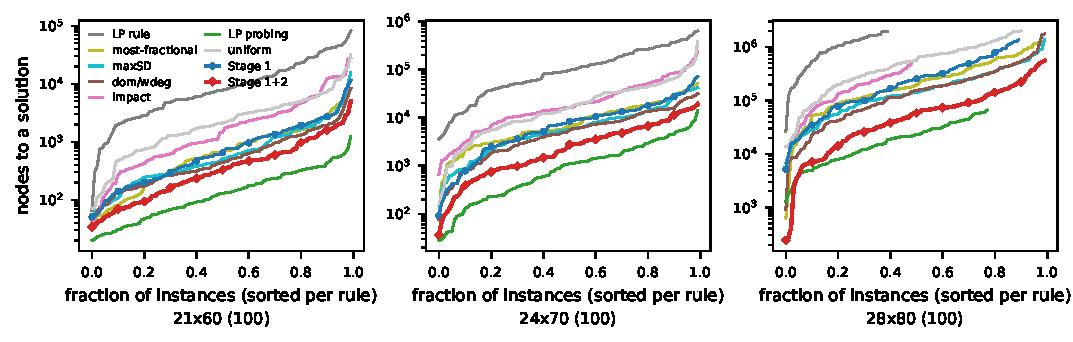
\includegraphics[width=\textwidth]{rq1_nodes.pdf}
\caption{Nodes to a solution on the three $100$-instance sets, each rule's instances sorted separately; a curve below another is a smaller tree at every quantile. Only LP probing, at one relaxation per free variable per node, lies below the learned rule.}
\label{fig:rq1nodes}
\end{figure*}

\begin{figure*}[t]
\centering
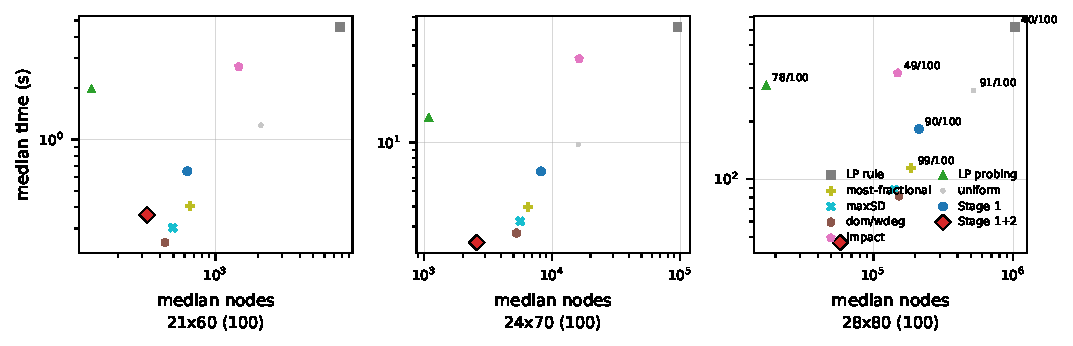
\includegraphics[width=\textwidth]{rq1_time.pdf}
\caption{Median nodes against median wall-clock per rule and size. Rules on one diagonal share a per-node cost; LP probing sits far above its node count, the learned rule slightly above the single-relaxation rules, and the vertical distance shrinks with size as the relaxation grows and the forward pass does not.}
\label{fig:rq1time}
\end{figure*}

\paragraph{Tree size.} Table~\ref{tab:rq1} and Figure~\ref{fig:rq1nodes} give the main result. At each of the three sizes the learned rule expands fewer nodes than every single-relaxation classical rule, and the paired tests are significant for every one of them: against the strongest cheap rule at each size (dom/wdeg at $21\times60$ and $24\times70$, maxSD at $28\times80$) the median per-instance ratio is $1.52\times$ ($p=0.035$), $1.79\times$ ($p=0.035$) and $3.20\times$ ($p=10^{-9}$); against most-fractional branching, the rule that a MIP solver uses when it has no pseudocosts, $2.27\times$, $3.67\times$ and $3.98\times$ ($p\le2\times10^{-4}$); against the most-integral LP rule, $24\times$ and $38\times$ at the two smaller sizes, while at $28\times80$ that rule solves $40/100$ instances within budget and expands $19\times$ more nodes on those (PAR-2 $1{,}688$ against $75$\,s).
The gains are distributional, not universal: the learned rule wins on $61$--$80$ of $100$ instances against the cheap rules, and loses on the rest. The one rule that builds a smaller tree is LP probing, by $2.7$--$2.9\times$ on the instances it solves, and it is the transplant of strong branching: it fixes every variable the relaxation can refute at every node, which is more information per node than any score, at $|K|$ relaxations per node. Stage~1 alone, the marginal rule without the cost-tuned order, expands $2.3\times$, $3.2\times$ and $5.0\times$ more nodes than the full rule at the three sizes (paired medians), is itself $12\times$ and $12\times$ below the LP rule at $21\times60$ and $24\times70$, is level with the cheap classical rules at $21\times60$ and behind them from $24\times70$ on, and leaves $10$ of the $28\times80$ instances unsolved: the marginal alone is a competitive value signal and an ordinary variable score, and the cost-tuned order is what moves the rule ahead of the field.

\paragraph{Wall-clock.} A smaller tree buys time only if the per-node cost allows, and Table~\ref{tab:profile} measures that cost by instrumenting whole trees. A single-relaxation rule's node costs $0.47$, $0.55$ and $0.61$\,ms at the three sizes, $90\%$ of it in the warm-started relaxation; the learned rule's node costs $0.71$, $0.73$ and $0.82$\,ms, of which the forward pass is $28$--$32\%$ and the relaxation $57$--$62\%$. The overhead ratio is therefore $1.5\times$ at $n=60$ and $1.3\times$ at $n=70$ and $80$, because the forward pass grows more slowly with size than the relaxation, while the node advantage rises from $1.5\times$ to $3.2\times$; wall-clock follows (Figure~\ref{fig:rq1time}, Table~\ref{tab:rq1}). At $21\times60$ the learned rule is as fast as most-fractional and maxSD branching and slower than dom/wdeg ($0.83\times$, $p=0.021$); at $24\times70$ it is faster than most-fractional ($2.4\times$, $p=4\times10^{-4}$) and maxSD ($1.5\times$, $p=0.004$) and level with dom/wdeg; at $28\times80$ it is faster than all of them, by $3.1\times$, $2.4\times$ and $2.0\times$ ($p\le0.002$), with $100/100$ solved against $99$ for most-fractional and $91$ for uniform branching and the lowest PAR-2 of the field. LP probing pays $13$--$18$\,ms per node, one relaxation per free variable, and is $5$--$8\times$ slower than the learned rule at the three sizes despite its smaller tree; at $28\times80$ it leaves $22$ instances unsolved (PAR-2 $820$ against $75$\,s). Impact-based search, which also probes, is $7\times$ slower than the learned rule at $21\times60$ and $19\times$ at $24\times70$ while expanding $6$--$9\times$ the nodes (paired medians), and at $28\times80$ it solves $49/100$ (PAR-2 $1{,}428$\,s).
At the two small sizes ($10\times25$, $18\times50$; $30$ instances, trees of $14$--$120$ nodes) every rule is within a few hundredths of a second and the learned rule is the slowest at $10\times25$, where a $14$-node tree cannot amortise $14$ forward passes; those sizes are reported in Appendix~\ref{app:small} and are not where the question is decided.

\paragraph{Reference signals.} Two rules in Table~\ref{tab:arms} are not deployable and bound what a value signal can do. The oracle, which enumerates $\SOL(F,\mathbf{v})$ at every node and branches on the most confident exact marginal, expands $22$ nodes at $10\times25$ against $21$ for the Stage-1 network, $14$ for the cost-tuned rule and $15.5$ for dom/wdeg: the exact value signal under the confidence rule is no better than its learned approximation and worse than a classical variable score, so the remaining headroom is in the variable choice, which is what Stage~2 addresses. Belief-propagation marginals, the NSNet transplant, give trees the size of Stage~1's at $18\times50$ ($118$ against $116$ nodes) at $35$\,ms per estimate against $0.3$--$0.5$\,ms for a dense forward pass, $50\times$ the wall-clock of the learned rule; the marginal network is this signal at a fraction of its price, and it is run once per node, which message passing at this cost cannot be. NSNet's own way of using a marginal, decoding one root estimate into an initial assignment for an incomplete local search, was also run: a WalkSAT-style search over $\{0,1\}^n$ on the residual $\|A\mathbf{x}-\mathbf{b}\|_1$ solves all $100$ instances at $21\times60$ in $1.2$--$1.5$\,s, $3$--$4\times$ the time of the learned search, and takes the same time whether its initial assignment comes from the marginal network, from LP rounding or from a uniform draw, so at this size the marginal buys the local search nothing and the comparison is between the two searches, not the two uses of the signal.

\subsection{RQ2: generalisation to larger instances}
\label{sec:rq2}

\begin{figure*}[t]
\centering
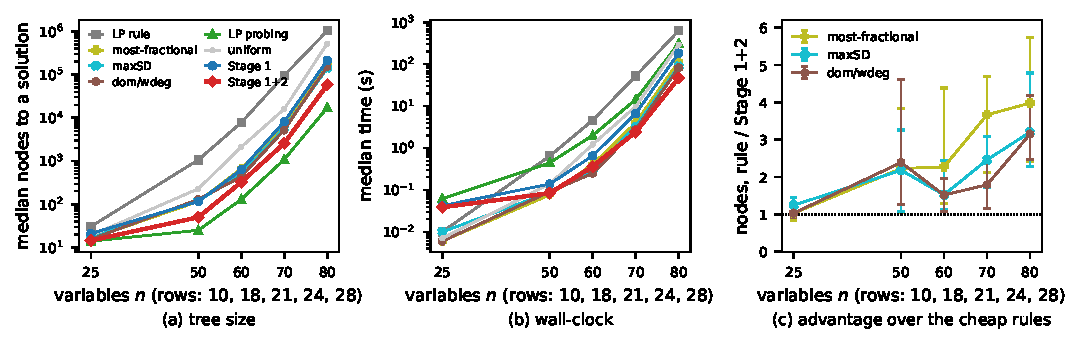
\includegraphics[width=\textwidth]{rq2_scaling.pdf}
\caption{Scaling with size at $p=0.3$. (a) Median nodes and (b) median wall-clock per rule ($30$ instances at $n=25,50$; $100$ at $n=60,70,80$). (c) Median per-instance node ratio of each cheap classical rule to the learned rule with $95\%$ bootstrap intervals; Stage~1 was trained at $n=25$ and Stage~2 at $n=60$, so $n=70$ and $80$ are extrapolation.}
\label{fig:rq2}
\end{figure*}

Both stages were trained below the sizes that matter: the marginal network on $10\times25$ states and the branching order on $21\times60$ states, with the architecture size-free (a graph network over the reduced instance) and the training signals defined at any size. Figure~\ref{fig:rq2} and Table~\ref{tab:rq1} answer the question in two parts. First, the rule transfers: at $24\times70$ and $28\times80$, sizes neither stage saw, it solves every instance within budget and keeps a significant node advantage over every single-relaxation rule. Second, the advantage grows with size rather than decaying: the node ratio against the strongest cheap rule rises from $1.5\times$ at $n=60$ to $1.8\times$ at $70$ and $3.2\times$ at $80$, against most-fractional branching from $2.3\times$ to $3.7\times$ and $4.0\times$, and the wall-clock ratio against dom/wdeg crosses one between $n=60$ ($0.83\times$) and $70$ ($1.09\times$) and reaches $2.0\times$ at $80$. The mechanism is the one of Figure~\ref{fig:rq1time}: the per-node premium of the forward pass is fixed while the relaxation and the tree grow, so a constant-factor node advantage becomes a time advantage once the tree is large enough, and the node advantage itself is larger where the search is longer, which Section~\ref{sec:rq3} traces to how the cost-tuned order refutes wrong values. The density sweep of Table~\ref{tab:density} shows the same ordering of sizes at $p=0.4$ and the collapse of every rule to the propagation floor at $p=0.2$, so the growth is a property of tree size and not of one density, although only $p=0.3$ is claimed here. The transfer is also uneven between the stages: Stage~1 alone keeps its node advantage over the LP rule at every size but falls behind the cheap classical rules in time from $24\times70$ and in solve rate at $28\times80$ ($90/100$), so what transfers usefully is the combination, with Stage~2's gain over Stage~1 growing from $2.3\times$ at $n=60$ to $5.0\times$ at $n=80$. What transfer does not do is extend the useful window: at $n=100$ no rule solves an instance within budget, and the next size would need either a cheaper node or clause learning.

\subsection{RQ3: are the two signals interchangeable, and is each stage necessary?}
\label{sec:rq3}
\label{sec:ablation}

\begin{table*}[t]
\centering
\caption{Value $\times$ variable cross ablation at $p=0.3$: each arm combines one variable-selection score with one first-value rule; everything else is identical. Columns per size: median nodes and the median per-instance node ratio to Stage~1+2 with bootstrap interval and sign-test $p$-value.}
\label{tab:cross}
\scriptsize
\begin{tabular}{lrlrlrl}
\toprule
 & \multicolumn{2}{c}{$21\times60$ (100)} & \multicolumn{2}{c}{$24\times70$ (100)} & \multicolumn{2}{c}{$28\times80$ (100)} \\
\cmidrule(lr){2-3}\cmidrule(lr){4-5}\cmidrule(lr){6-7}
variable, value & nodes & ratio & nodes & ratio & nodes & ratio \\
\midrule
LP var., LP value (LP rule) & 7,762 & 23.90$\times$ [15.11, 37.29] $10^{-25}$ & 95,440 & 37.74$\times$ [27.17, 66.01] $8\cdot10^{-27}$ & 1,029,039 & 19.25$\times$ [13.83, 27.87] $10^{-9}$ \\
LP var., S1 value & 9,810 & 27.87$\times$ [19.53, 36.44] $10^{-21}$ & 69,872 & 39.45$\times$ [20.99, 58.92] $10^{-21}$ & 647,145 & 16.32$\times$ [6.86, 23.92] $9\cdot10^{-5}$ \\
S1 var., S1 value (Stage 1) & 628 & 2.32$\times$ [1.08, 3.25] $0.01$ & 8,174 & 3.17$\times$ [2.32, 4.40] $10^{-6}$ & 212,271 & 5.01$\times$ [3.01, 6.62] $9\cdot10^{-11}$ \\
S1 var., LP value & 956 & 2.84$\times$ [1.77, 3.75] $5\cdot10^{-6}$ & 6,998 & 3.28$\times$ [2.56, 4.22] $6\cdot10^{-7}$ & 278,175 & 5.85$\times$ [4.04, 8.77] $5\cdot10^{-12}$ \\
S2 var., S1 value (Stage 1+2) & 325 & --- & 2,580 & --- & 58,026 & --- \\
S2 var., LP value & 292 & 0.79$\times$ [0.60, 1.04] $0.09$ & 2,348 & 1.19$\times$ [0.91, 1.66] $0.27$ & 69,665 & 1.41$\times$ [1.03, 1.86] $0.09$ \\
\bottomrule
\end{tabular}
\end{table*}

\begin{figure*}[t]
\centering
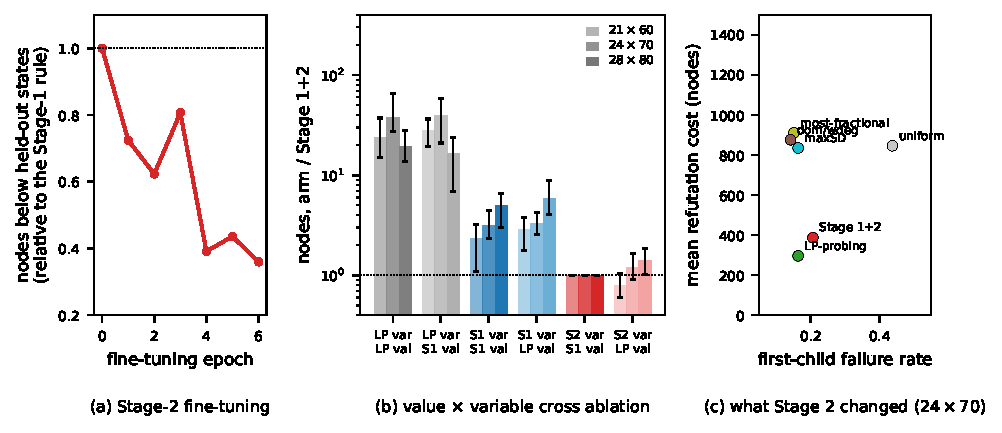
\includegraphics[width=\textwidth]{rq3.pdf}
\caption{(a) Stage-2 fine-tuning at $p=0.3$: nodes below $150$ held-out training states relative to the Stage-1 rule, by epoch; epoch $6$ is selected. (b) The cross ablation of Table~\ref{tab:cross} as node ratios to Stage~1+2 (log scale, $95\%$ bootstrap intervals). (c) Refutation structure at $24\times70$: how often a rule's first value is refuted against what a refutation costs it; the cost-tuned rule is wrong more often and pays far less per mistake.}
\label{fig:rq3}
\end{figure*}

\paragraph{Value and variable are separable, and the variable carries the gain.} Table~\ref{tab:cross} and Figure~\ref{fig:rq3}b combine each of three variable-selection scores (LP most-integral, Stage-1 confidence, Stage-2 cost-tuned) with each of two first-value rules (LP rounding, Stage-1 marginal). Reading the table by column, the variable score is decisive: with the Stage-1 value fixed, moving the variable score from LP to Stage~1 to Stage~2 divides the tree by $12\times$ and then $2.3\times$ at $21\times60$, and the LP variable with the exact-trained marginal value is $28\times$ worse than the full rule, $37\times$ at $24\times70$, and solves $26/100$ instances at $28\times80$ where the full rule solves all. Reading it by row, the value rule is not: with the Stage-2 variable fixed, replacing the marginal value by LP rounding changes the tree by $0.79\times$ ($p=0.09$) at $21\times60$, $1.19\times$ ($p=0.27$) at $24\times70$ and $1.41\times$ ($p=0.09$) at $28\times80$, none significant at the $5\%$ level, although the direction turns in favour of the marginal value as the tree grows; with the Stage-1 variable fixed the LP value costs $1.5\times$ and $1.3\times$ more nodes at the two smaller sizes, and that arm falls further behind the full rule with size ($2.8\times$, $3.3\times$, $5.9\times$), which is the Stage-2 gain growing with the tree.
Two conclusions follow, one of them against the design of Section~\ref{sec:method}. The signals are not interchangeable in the sense that matters: the marginal-trained network is what makes a good variable score possible, through its trunk and through the confidence score that Stage~2 starts from, and no amount of value accuracy rescues the LP variable choice. But the exact-marginal \emph{value} is replaceable at this density: once the variable is chosen by the cost-tuned score, rounding the relaxation gives a tree that is not significantly different at any size, and at most $1.4\times$ larger at $28\times80$, which is consistent with Section~\ref{sec:rq1}'s oracle result that even exact marginals under the confidence rule do not beat a classical variable score. The value signal's job in this method is to train the representation, not to pick values.

\paragraph{What Stage 2 learned.} The fine-tuning changes the search in a way that the per-instance records make visible (Figure~\ref{fig:rq3}c; the full table is in Appendix~\ref{app:trace}). For every rule we record, on the path to the solution, how often the first value tried was refuted (the subtree under it exhausted) and what each such refutation cost. The Stage-1 confidence rule is wrong least often ($6\%$ of its decisions at $21\times60$) and pays most per mistake ($246$ nodes); the cost-tuned rule is wrong three times as often ($19\%$) and pays a quarter per mistake ($65$ nodes), and its solution path is shorter ($28$ against $46$ decisions) because the variables it picks trigger more propagation and relaxation fixings. The same holds against the classical rules at $24\times70$: dom/wdeg, maxSD and most-fractional branching are refuted on $14$--$16\%$ of their decisions at $835$--$911$ nodes each, the learned rule on $21\%$ at $387$. This is fail-first \citep{haralick1980increasing} learned from the cost signal rather than designed: the policy moves away from the variables it is surest about towards variables whose wrong value is cheap to exhaust, and the arm that keeps the Stage-2 variable with the LP value has the same profile ($16\%$, $63$ nodes), so the structure comes from the variable choice.

\begin{table*}[t]
\centering
\caption{Training variants at $p=0.3$: median nodes and median per-instance node ratio to the reference Stage~1+2 rule, per size. Stage-1 variants are run with the confidence rule (no Stage 2); Stage-2 variants share the frozen reference trunk unless stated.}
\label{tab:variants}
\scriptsize
\begin{tabular}{lrlrlrl}
\toprule
 & \multicolumn{2}{c}{$21\times60$ (100)} & \multicolumn{2}{c}{$24\times70$ (100)} & \multicolumn{2}{c}{$28\times80$ (100)} \\
\cmidrule(lr){2-3}\cmidrule(lr){4-5}\cmidrule(lr){6-7}
variant & nodes & ratio & nodes & ratio & nodes & ratio \\
\midrule
Stage 1 (reference) & 628 & 2.32$\times$ [1.08, 3.25] $0.01$ & 8,174 & 3.17$\times$ [2.32, 4.40] $10^{-6}$ & 212,271 (90/100) & 5.01$\times$ [3.01, 6.62] $9\cdot10^{-11}$ \\
Stage 1, hard $0/1$ labels & 848 & 2.66$\times$ [1.93, 4.05] $3\cdot10^{-5}$ & 7,644 & 2.73$\times$ [2.03, 3.98] $4\cdot10^{-9}$ & 259,605 (95/100) & 4.18$\times$ [3.26, 6.63] $10^{-12}$ \\
Stage 1, training seed 1 & 562 & 1.72$\times$ [1.17, 2.49] $4\cdot10^{-3}$ & 7,318 & 2.72$\times$ [1.60, 4.60] $4\cdot10^{-4}$ & 207,117 (91/100) & 4.03$\times$ [2.63, 5.13] $10^{-10}$ \\
Stage 1, training seed 2 & 553 & 1.65$\times$ [1.10, 2.14] $0.04$ & 6,199 & 2.06$\times$ [1.01, 2.76] $0.09$ & 213,055 (95/100) & 4.37$\times$ [3.09, 6.74] $3\cdot10^{-11}$ \\
Stage 1, $2{,}771$ states (size ctrl.) & 662 & 2.22$\times$ [1.47, 2.61] $8\cdot10^{-5}$ & 6,897 & 3.89$\times$ [1.96, 6.15] $3\cdot10^{-5}$ & 168,442 (91/100) & 4.12$\times$ [3.08, 6.44] $10^{-9}$ \\
Stage 1 on $21\times60$ states (M1) & 912 & 2.44$\times$ [1.64, 4.10] $10^{-5}$ & 10,754 & 3.94$\times$ [2.51, 7.91] $10^{-7}$ & 225,182 (85/100) & 5.73$\times$ [2.99, 7.19] $8\cdot10^{-8}$ \\
Stage 1, NSNet architecture & 892 & 2.75$\times$ [2.02, 4.03] $10^{-7}$ & 12,500 & 5.02$\times$ [3.46, 7.46] $5\cdot10^{-13}$ & 248,556 (70/100) & 4.75$\times$ [3.45, 7.73] $10^{-8}$ \\
\midrule
Stage 1+2 (reference) & 325 & --- & 2,580 & --- & 58,026 & --- \\
Stage 2 from a random head & 333 & 1.04$\times$ [0.74, 1.28] $0.92$ & 1,878 & 0.86$\times$ [0.65, 1.10] $0.27$ & 59,122 (99/100) & 1.03$\times$ [0.94, 1.20] $0.84$ \\
Stage 2 from the LP rule & 376 & 1.06$\times$ [0.73, 1.31] $0.76$ & 3,024 & 0.86$\times$ [0.62, 1.39] $0.48$ & 72,539 & 1.12$\times$ [0.87, 1.48] $0.37$ \\
Stage 2, trunk unfrozen & 280 & 0.76$\times$ [0.56, 1.20] $0.37$ & 2,427 & 0.83$\times$ [0.69, 1.12] $0.37$ & 59,692 & 1.06$\times$ [0.70, 1.65] $0.76$ \\
Stage 1+2 trained at $p=0.5$ & 379 & 1.32$\times$ [1.00, 1.68] $0.09$ & 4,096 & 1.64$\times$ [1.16, 2.35] $7\cdot10^{-3}$ & 80,002 & 1.76$\times$ [1.44, 2.52] $4\cdot10^{-3}$ \\
\bottomrule
\end{tabular}
\end{table*}

\paragraph{Is each stage necessary, and which parts of the recipe matter?} Table~\ref{tab:variants} varies the training of each stage with everything else fixed. For Stage~1, nothing in the recipe moves the value accuracy: the label form (soft marginals against the planted $0/1$ solution), the training seed and the number of training states ($10{,}000$ against $2{,}771$) change the test accuracy on $\FORCED$ variables by at most $0.2$ points ($79.0$--$79.2\%$ against a ceiling of $83.3\%$), a network of the NSNet architecture \citep{li2022nsnet} trained on the same states reaches $80.4\%$, and training on $21\times60$ states instead of $10\times25$ (M1) raises accuracy on $21\times60$ states by $2.4$ points. The trees tell a different story. Two training seeds of the reference recipe expand $553$ and $562$ nodes at $21\times60$ against the reference's $628$, so the Stage-1 rule carries a seed variance of about $\pm10\%$ that no label or architecture choice exceeds in the right direction; the two networks with the \emph{higher} value accuracy, M1 and the NSNet architecture, expand the \emph{largest} trees ($912$ and $892$ at $21\times60$; $10{,}754$ and $12{,}500$ at $24\times70$ against $6{,}199$--$8{,}175$ for the reference recipe) and at $28\times80$ solve the fewest instances within budget ($85$ and $70$ of $100$, against $91$--$95$ for the other Stage-1 variants and $100$ for the full rule); every Stage-1 variant expands $4.0$--$5.7\times$ the nodes of the full rule there.
Value accuracy and tree size are therefore not the same quantity, which is the point of Table~\ref{tab:cross} seen from the other side, and the Stage-1 recipe is necessary only in the sense that any of these networks supplies a trunk and a confidence score that Stage~2 then improves by $2$--$3\times$.
For Stage~2 the recipe matters less than we had designed it to. Starting the policy head at random, which is what reinforcement learning from scratch would do with this trunk, leaves the initial policy at $7\times$ the root cost of the marginal rule, and six epochs later it is level with the reference ($1.04\times$, $0.86\times$ and $1.03\times$ at the three sizes, none significant); starting it from the LP rule ends in the same place ($1.06\times$, $0.86\times$, $1.12\times$). Unfreezing the trunk makes the held-out node count diverge from the third epoch (to $2.7$--$5.4\times$ the Stage-1 rule's), but the checkpoint that epoch selection keeps, from the first epoch, is as good as the frozen one ($0.76\times$, $0.83\times$, $1.06\times$, not significant). The frozen trunk is thus what keeps the fine-tuning stable enough to continue, and what lets the gain be attributed to the order; it is not a source of tree size, and we do not claim one. A policy fine-tuned on $p=0.5$ data and deployed at $p=0.3$ expands $1.3\times$, $1.6\times$ and $1.8\times$ more nodes than the one trained in distribution ($p\le0.01$ at the two larger sizes), so the training density matters but does not decide the result.

\subsection{RQ4: against complete solvers}
\label{sec:rq4}

\begin{table*}[t]
\centering
\caption{Inside SCIP at $p=0.3$ (presolve, cuts and primal heuristics off, depth-first node selection, first solution stops): SCIP's own rules against the learned rule as a branching plug-in, with conflict analysis off and on. Ratios are rule / plug-in as in Table~\ref{tab:rq1}.}
\label{tab:scip}
\footnotesize
\begin{tabular}{llrrrll}
\toprule
conflict & rule & solved & med.\ nodes & med.\ s & nodes, rule / plug-in & time, rule / plug-in \\
\midrule
\multicolumn{7}{l}{\emph{$21\times60$ (100)}} \\
off & RPB (SCIP default) & 100/100 & 828 & 0.06 & 2.14$\times$ [1.57, 3.42] $5\cdot10^{-6}$ & 0.34$\times$ [0.24, 0.51] $6\cdot10^{-7}$ \\
off & most-fractional (SCIP) & 100/100 & 558 & 0.05 & 1.83$\times$ [1.37, 2.39] $10^{-4}$ & 0.26$\times$ [0.20, 0.39] $10^{-15}$ \\
off & inference (SCIP) & 100/100 & 767 & 0.06 & 2.41$\times$ [1.77, 3.80] $8\cdot10^{-5}$ & 0.32$\times$ [0.23, 0.45] $6\cdot10^{-11}$ \\
off & \textbf{Stage 1+2 plug-in} & 100/100 & \textbf{274} & 0.14 & --- & --- \\
\midrule
\multicolumn{7}{l}{\emph{$21\times60$ (100)}} \\
on & RPB (SCIP default) & 100/100 & 705 & 0.06 & 1.86$\times$ [1.46, 2.81] $3\cdot10^{-5}$ & 0.32$\times$ [0.25, 0.46] $10^{-9}$ \\
on & most-fractional (SCIP) & 100/100 & 528 & 0.04 & 1.69$\times$ [1.33, 2.27] $10^{-4}$ & 0.28$\times$ [0.23, 0.39] $10^{-11}$ \\
on & inference (SCIP) & 100/100 & 795 & 0.07 & 2.09$\times$ [1.62, 2.84] $10^{-5}$ & 0.33$\times$ [0.24, 0.45] $10^{-12}$ \\
on & \textbf{Stage 1+2 plug-in} & 100/100 & \textbf{256} & 0.14 & --- & --- \\
\midrule
\multicolumn{7}{l}{\emph{$24\times70$ (100)}} \\
off & RPB (SCIP default) & 100/100 & 7,010 & 0.56 & 3.47$\times$ [2.42, 6.00] $6\cdot10^{-11}$ & 0.83$\times$ [0.58, 1.37] $0.37$ \\
off & most-fractional (SCIP) & 100/100 & 5,026 & 0.40 & 3.47$\times$ [1.59, 4.23] $3\cdot10^{-5}$ & 0.86$\times$ [0.41, 0.98] $0.04$ \\
off & inference (SCIP) & 100/100 & 6,694 & 0.50 & 4.00$\times$ [2.48, 6.36] $10^{-9}$ & 0.95$\times$ [0.60, 1.37] $0.48$ \\
off & \textbf{Stage 1+2 plug-in} & 100/100 & \textbf{1,915} & 0.61 & --- & --- \\
\midrule
\multicolumn{7}{l}{\emph{$24\times70$ (100)}} \\
on & RPB (SCIP default) & 100/100 & 5,496 & 0.49 & 3.06$\times$ [2.57, 4.53] $6\cdot10^{-7}$ & 0.80$\times$ [0.64, 1.05] $0.13$ \\
on & most-fractional (SCIP) & 100/100 & 5,340 & 0.50 & 2.98$\times$ [1.67, 3.87] $10^{-5}$ & 0.74$\times$ [0.48, 1.03] $0.13$ \\
on & inference (SCIP) & 100/100 & 5,578 & 0.48 & 3.12$\times$ [2.26, 4.34] $10^{-9}$ & 0.78$\times$ [0.58, 0.97] $0.02$ \\
on & \textbf{Stage 1+2 plug-in} & 100/100 & \textbf{1,806} & 0.60 & --- & --- \\
\midrule
\multicolumn{7}{l}{\emph{$28\times80$ (100)}} \\
off & RPB (SCIP default) & 100/100 & 224,088 & 25.05 & 3.83$\times$ [2.36, 5.96] $10^{-10}$ & 1.11$\times$ [0.71, 1.73] $0.48$ \\
off & most-fractional (SCIP) & 100/100 & 136,840 & 15.84 & 2.11$\times$ [1.63, 3.01] $7\cdot10^{-3}$ & 0.66$\times$ [0.49, 0.93] $0.02$ \\
off & inference (SCIP) & 100/100 & 232,221 & 25.19 & 3.90$\times$ [3.00, 5.70] $10^{-10}$ & 1.14$\times$ [0.84, 1.59] $0.62$ \\
off & \textbf{Stage 1+2 plug-in} & 100/100 & \textbf{60,174} & 22.42 & --- & --- \\
\midrule
\multicolumn{7}{l}{\emph{$28\times80$ (100)}} \\
on & RPB (SCIP default) & 100/100 & 148,872 & 19.75 & 2.43$\times$ [1.80, 4.76] $3\cdot10^{-5}$ & 0.77$\times$ [0.57, 1.43] $0.37$ \\
on & most-fractional (SCIP) & 100/100 & 128,310 & 17.10 & 2.08$\times$ [1.30, 2.76] $10^{-3}$ & 0.68$\times$ [0.41, 0.96] $0.06$ \\
on & inference (SCIP) & 100/100 & 122,144 & 14.62 & 2.36$\times$ [1.52, 3.00] $10^{-4}$ & 0.71$\times$ [0.46, 0.90] $0.01$ \\
on & \textbf{Stage 1+2 plug-in} & 100/100 & \textbf{58,564} & 24.00 & --- & --- \\
\bottomrule
\end{tabular}
\end{table*}

\paragraph{As a branching rule inside SCIP.} The learned rule is a function of the reduced instance and its relaxation vertex, so it can be installed as a branching rule in a MIP solver. We implemented it as a PySCIPOpt branching plug-in and ran SCIP \citep{bestuzheva2021scip} on the same instances with presolve, cutting planes and primal heuristics off, depth-first node selection and a stop at the first solution, so that SCIP's search is the one our loop performs with SCIP's propagation and LP in place of ours; conflict analysis, which our loop lacks, is run both off and on. The comparison is against reliability pseudocost branching (RPB, SCIP's default and the rule the learning-to-branch literature imitates, \citealp{achterberg2005branching}), SCIP's most-fractional rule and its inference rule. Table~\ref{tab:scip} shows the node advantage survives the change of engine and the addition of clause learning: on the $100$-instance sets the plug-in expands $1.9$--$3.8\times$ fewer nodes than RPB at every size with conflict analysis off or on (sign test $p\le3\times10^{-5}$ throughout), and $1.7$--$4.0\times$ fewer than SCIP's most-fractional and inference rules. Time is a draw against RPB and a loss against the cheapest rule: the forward pass is $60$--$80\%$ of the branching callback, so the plug-in is $3\times$ slower than every SCIP rule at $21\times60$, where trees are a few hundred nodes, while at $24\times70$ and $28\times80$ its median time is within $0.8$--$1.1\times$ of RPB's with conflict analysis off or on (no paired difference significant) and $0.66$--$0.86\times$ behind SCIP's most-fractional rule ($p=0.02$--$0.06$). Inside a solver the answer to RQ1 therefore splits: the learned rule is the better branching rule by tree size at every size, matches the solver's default rule in time once the tree is large enough to amortise the forward pass, and does not beat the cheapest rule in time.

\begin{table}[t]
\centering
\caption{End to end at $p=0.3$, same instances and budgets, single-threaded: complete solvers with all defaults, lattice reduction with bounded enumeration, and the learned search. Median time over solved instances and PAR-2; node counts are not comparable across engines and are omitted.}
\label{tab:e2e}
\footnotesize
\fitc{\begin{tabular}{lrrr}
\toprule
method & solved & med.\ s & PAR-2 s \\
\midrule
\multicolumn{4}{l}{\emph{$21\times60$ (100)}} \\
SCIP (all defaults) & 100/100 & 0.35 & 0.5 \\
CP-SAT (1 worker) & 100/100 & 0.04 & 0.1 \\
Gurobi (1 thread) & 100/100 & 0.04 & 0.1 \\
BKZ-40 $\times$ 30 + enumeration & 100/100 & 0.20 & 0.4 \\
\textbf{Stage 1+2 (our loop)} & 100/100 & 0.36 & 0.6 \\
\midrule
\multicolumn{4}{l}{\emph{$24\times70$ (100)}} \\
SCIP (all defaults) & 100/100 & 2.33 & 2.5 \\
CP-SAT (1 worker) & 100/100 & 0.36 & 0.6 \\
Gurobi (1 thread) & 100/100 & 0.31 & 0.4 \\
BKZ-40 $\times$ 30 + enumeration & 100/100 & 13.20 & 11.5 \\
\textbf{Stage 1+2 (our loop)} & 100/100 & 2.39 & 3.6 \\
\midrule
\multicolumn{4}{l}{\emph{$28\times80$ (100)}} \\
SCIP (all defaults) & 100/100 & 16.47 & 21.1 \\
CP-SAT (1 worker) & 100/100 & 12.24 & 39.8 \\
Gurobi (1 thread) & 100/100 & 6.61 & 9.8 \\
BKZ-40 $\times$ 30 + enumeration & 100/100 & 124.90 & 117.7 \\
\textbf{Stage 1+2 (our loop)} & 100/100 & 46.61 & 74.5 \\
\bottomrule
\end{tabular}}
\end{table}

\paragraph{End to end.} Table~\ref{tab:e2e} places the learned search next to complete solvers with all their defaults (Gurobi with one thread \citep{gurobi2024}; CP-SAT with one worker \citep{perron2023ortools}; SCIP with presolve, cuts, heuristics, conflict analysis and RPB) and next to lattice reduction with bounded enumeration (BKZ block $40$, $30$ column permutations, fpylll enumeration \citep{fpylll2023} with a $300$\,s cap), on the same instances and budgets. Every method solves every instance. Gurobi is the fastest at every size ($0.05$, $0.31$ and $6.6$\,s median at $n=60$, $70$, $80$) and CP-SAT the next ($0.04$, $0.36$, $12.2$\,s, with a heavier tail at $28\times80$); SCIP with its defaults is level with the learned search at $24\times70$ ($2.33$ against $2.39$\,s) and $2.8\times$ faster at $28\times80$ ($16.5$ against $46.6$\,s). Lattice enumeration solves the $21\times60$ set in $0.2$\,s per instance but its cost grows faster than the search's: $13.2$\,s at $24\times70$ and $125$\,s at $28\times80$, $5.5\times$ and $2.7\times$ slower than the learned search.
Two things are true at once. The learned search is not the fastest way to solve these instances: a commercial MIP solver and a CP-SAT solver with presolve and clause learning are ahead by one to two orders of magnitude at $n\le70$ and by $4$--$7\times$ at $n=80$, and SCIP is ahead at the largest size. And none of that bears on the branching question: the comparison that isolates the branching decision is Table~\ref{tab:rq1}, and inside SCIP the decision quality carries over while the per-node cost does not. The honest summary is that this paper improves the branching rule, in its own loop and inside SCIP, and does not by itself produce a faster solver; the gap to the solvers is presolve, clause learning and a compiled node, none of which the learned rule addresses.

\section{Conclusion}
\label{sec:conclusion}

A branching decision asks two questions, and this paper trained on an exact answer to each: the conditional marginal, enumerable where solutions can be enumerated and carried to every node by the reduction identity, for which value to try; and the number of nodes below a decision, produced by the search as it backtracks, for which variable to branch on. Against seven classical rules and the transplants of three learned-branching families, in one search loop, on $100$-instance sets at one density, the learned rule expands the fewest nodes of any single-relaxation rule at every size and is also the fastest at $28\times80$; trained at $n\le60$, its advantage grows with size rather than decaying; and it carries its node advantage into SCIP against reliability branching with conflict analysis on or off. The ablations say what the recipe is: the variable choice carries the gain, the cost-tuned order is fail-first learned rather than designed, the frozen marginal trunk is what keeps the fine-tuning stable, and the exact-marginal value, the ingredient the method was named for, turns out to be replaceable by LP rounding once the variable is chosen well, with at most a $1.4\times$ difference at the largest size.

Three limitations bound the result. The claims are for one density, chosen because the gap is largest there, and we have shown that at the market-split density the learned rule and most-fractional branching are indistinguishable. The learned search is not competitive end to end: Gurobi, CP-SAT and SCIP with their defaults are faster, by orders of magnitude at $n\le70$, so the contribution is to the branching rule and not to the solver; lattice enumeration also solves every instance we study, though at the two larger sizes it is slower than the learned search. And exact supervision bounds Stage~1 to sizes that enumerate, so the value signal cannot be trained where it is deployed; that it does not need to be, because the LP value serves, is the one result that eases this.

The next steps follow from the negative results. If the value signal's job is to train the representation, a cheaper target than exact marginals may do, and Stage~2's cost signal needs no enumeration at all, so the order can be fine-tuned at sizes where enumeration fails and, since the number of nodes below a decision is defined whether or not the subtree holds a solution, on infeasible instances, which this paper excludes. The time gap inside a solver is a forward-pass budget: the plug-in loses on time with the network at $64$--$80\%$ of the callback, so either a smaller network or a learned rule evaluated at a subset of nodes is the route to a rule that wins on both counts.

\appendix
\section{The two small sizes}
\label{app:small}
\begin{table}[t]
\centering
\caption{The two small sizes ($30$ instances each): same columns as Table~\ref{tab:rq1}. Trees are tens of nodes and no rule separates from the others in time except through the cost of its score.}
\label{tab:small}
\footnotesize
\fitc{\begin{tabular}{lrrrrll}
\toprule
rule & solved & med.\ nodes & med.\ s & PAR-2 s & nodes, rule / Stage 1+2 & time, rule / Stage 1+2 \\
\midrule
\multicolumn{7}{l}{\emph{10$\times$25 (30), budget 60\,s}} \\
LP rule (most-integral) & 30/30 & 30 & 0.01 & 0.0 & 1.89$\times$ [1.53, 2.23] $7\cdot10^{-9}$ & 0.23$\times$ [0.20, 0.28] $10^{-9}$ \\
most-fractional & 30/30 & 16 & 0.01 & 0.0 & 1.03$\times$ [0.83, 1.18] $0.70$ & 0.16$\times$ [0.13, 0.17] $10^{-9}$ \\
maxSD & 30/30 & 18 & 0.01 & 0.0 & 1.24$\times$ [1.18, 1.46] $10^{-5}$ & 0.27$\times$ [0.20, 0.30] $10^{-9}$ \\
dom/wdeg & 30/30 & 16 & 0.01 & 0.0 & 1.03$\times$ [0.93, 1.19] $0.85$ & 0.16$\times$ [0.12, 0.18] $10^{-9}$ \\
impact & 30/30 & 17 & 0.03 & 0.0 & 1.14$\times$ [1.07, 1.28] $0.02$ & 0.75$\times$ [0.67, 0.89] $6\cdot10^{-5}$ \\
LP probing & 30/30 & 14 & 0.06 & 0.1 & 0.94$\times$ [0.81, 1.07] $0.34$ & 1.43$\times$ [1.28, 1.63] $10^{-4}$ \\
uniform & 30/30 & 19 & 0.01 & 0.0 & 1.23$\times$ [1.10, 1.41] $10^{-4}$ & 0.19$\times$ [0.15, 0.21] $10^{-9}$ \\
oracle marginals & 30/30 & 22 & 0.19 & 0.2 & 1.47$\times$ [1.39, 1.63] $10^{-9}$ & 4.52$\times$ [4.14, 5.41] $10^{-9}$ \\
BP marginals (NSNet-based) & 30/30 & 21 & 0.41 & 0.4 & 1.47$\times$ [1.32, 1.63] $4\cdot10^{-9}$ & 10.06$\times$ [9.01, 11.44] $10^{-9}$ \\
Stage 1 & 30/30 & 21 & 0.04 & 0.0 & 1.45$\times$ [1.30, 1.55] $4\cdot10^{-9}$ & 1.10$\times$ [1.05, 1.14] $0.02$ \\
\textbf{Stage 1+2} & 30/30 & \textbf{14} & \textbf{0.04} & 0.0 & --- & --- \\
\midrule
\multicolumn{7}{l}{\emph{18$\times$50 (30), budget 300\,s}} \\
LP rule (most-integral) & 30/30 & 1,066 & 0.64 & 0.9 & 13.89$\times$ [7.69, 42.45] $10^{-9}$ & 4.71$\times$ [3.68, 12.60] $9\cdot10^{-7}$ \\
most-fractional & 30/30 & 116 & 0.08 & 0.1 & 2.23$\times$ [1.04, 3.83] $0.10$ & 0.82$\times$ [0.62, 1.12] $0.36$ \\
maxSD & 30/30 & 120 & 0.09 & 0.1 & 2.18$\times$ [1.07, 3.26] $0.04$ & 0.93$\times$ [0.74, 1.33] $0.58$ \\
dom/wdeg & 30/30 & 130 & 0.09 & 0.1 & 2.39$\times$ [1.27, 4.62] $0.02$ & 0.90$\times$ [0.52, 1.89] $1.00$ \\
impact & 30/30 & 315 & 0.49 & 0.7 & 4.93$\times$ [3.26, 8.41] $9\cdot10^{-7}$ & 5.36$\times$ [3.57, 8.12] $6\cdot10^{-8}$ \\
LP probing & 30/30 & 25 & 0.44 & 0.5 & 0.55$\times$ [0.44, 0.70] $6\cdot10^{-5}$ & 5.36$\times$ [4.21, 6.34] $10^{-9}$ \\
uniform & 30/30 & 228 & 0.14 & 0.3 & 3.86$\times$ [2.12, 8.05] $3\cdot10^{-4}$ & 1.55$\times$ [0.94, 2.72] $0.10$ \\
BP marginals (NSNet-based) & 30/30 & 118 & 4.12 & 6.1 & 1.85$\times$ [1.12, 3.22] $0.04$ & 50.13$\times$ [34.89, 64.65] $10^{-9}$ \\
Stage 1 & 30/30 & 116 & 0.14 & 0.2 & 1.88$\times$ [1.01, 2.93] $0.06$ & 1.40$\times$ [1.24, 2.08] $5\cdot10^{-3}$ \\
\textbf{Stage 1+2} & 30/30 & \textbf{50} & \textbf{0.08} & 0.1 & --- & --- \\
\bottomrule
\end{tabular}}
\end{table}
Table~\ref{tab:small} reports $10\times25$ and $18\times50$. The reference signals appear here because the oracle enumerates $\SOL(F,\mathbf{v})$ at every node and is affordable only at $10\times25$, and belief propagation finishes within budget at $18\times50$.

\section{Refutation structure of every rule}
\label{app:trace}
\begin{table*}[t]
\centering
\caption{Refutation structure per rule at $p=0.3$ (solved instances; medians over instances): nodes, decisions on the solution path, share of nodes in refuted subtrees, fraction of path decisions whose first value was refuted, mean cost of such a refutation, and the median depth of refuted decisions as a fraction of the path length.}
\label{tab:trace}
\scriptsize
\begin{tabular}{lrrrrrrr}
\toprule
rule & $n$ & nodes & path & refuted share & first-child failure & refutation cost & depth frac.\ \\
\midrule
\multicolumn{8}{l}{\emph{21$\times$60 (100)}} \\
LP rule & 100 & 7,762 & 41 & 0.995 & 0.111 & 1,677 & 0.42 \\
most-fractional & 100 & 662 & 40 & 0.940 & 0.135 & 121 & 0.27 \\
maxSD & 100 & 494 & 36 & 0.917 & 0.156 & 89 & 0.59 \\
dom/wdeg & 100 & 436 & 34 & 0.920 & 0.113 & 115 & 0.42 \\
impact & 100 & 1,464 & 31 & 0.973 & 0.412 & 98 & 0.54 \\
LP-probing & 100 & 130 & 17 & 0.809 & 0.125 & 44 & 0.80 \\
uniform & 100 & 2,112 & 40 & 0.981 & 0.432 & 129 & 0.56 \\
Stage 1 & 100 & 628 & 46 & 0.923 & 0.064 & 246 & 0.52 \\
Stage 1+2 & 100 & 325 & 28 & 0.908 & 0.185 & 65 & 0.62 \\
S1 var / LP val & 100 & 956 & 46 & 0.947 & 0.088 & 239 & 0.45 \\
S2 var / LP val & 100 & 292 & 25 & 0.909 & 0.160 & 63 & 0.37 \\
LP var / S1 val & 100 & 9,810 & 42 & 0.996 & 0.125 & 1,998 & 0.48 \\
\midrule
\multicolumn{8}{l}{\emph{24$\times$70 (100)}} \\
LP rule & 100 & 95,440 & 51 & 0.999 & 0.119 & 15,884 & 0.34 \\
most-fractional & 100 & 6,504 & 49 & 0.992 & 0.151 & 911 & 0.26 \\
maxSD & 100 & 5,637 & 44 & 0.991 & 0.163 & 835 & 0.53 \\
dom/wdeg & 100 & 5,263 & 42 & 0.992 & 0.141 & 876 & 0.38 \\
impact & 100 & 16,256 & 40 & 0.997 & 0.421 & 1,078 & 0.52 \\
LP-probing & 100 & 1,088 & 20 & 0.974 & 0.163 & 296 & 0.73 \\
uniform & 100 & 16,028 & 48 & 0.997 & 0.437 & 846 & 0.56 \\
Stage 1 & 100 & 8,174 & 56 & 0.993 & 0.070 & 2,136 & 0.46 \\
Stage 1+2 & 100 & 2,580 & 33 & 0.986 & 0.206 & 387 & 0.57 \\
S1 var / LP val & 100 & 6,998 & 55 & 0.992 & 0.103 & 1,319 & 0.45 \\
S2 var / LP val & 100 & 2,348 & 30 & 0.986 & 0.200 & 398 & 0.36 \\
LP var / S1 val & 100 & 69,872 & 50 & 0.999 & 0.134 & 9,734 & 0.45 \\
\midrule
\multicolumn{8}{l}{\emph{28$\times$80 (100)}} \\
LP rule & 40 & 1,029,039 & 59 & 1.000 & 0.126 & 137,471 & 0.28 \\
most-fractional & 99 & 187,381 & 58 & 1.000 & 0.173 & 21,053 & 0.21 \\
maxSD & 100 & 141,178 & 52 & 1.000 & 0.206 & 13,784 & 0.47 \\
dom/wdeg & 100 & 152,598 & 50 & 1.000 & 0.179 & 17,945 & 0.27 \\
impact & 49 & 149,624 & 49 & 1.000 & 0.432 & 7,945 & 0.49 \\
LP-probing & 78 & 17,148 & 22 & 0.998 & 0.222 & 3,594 & 0.60 \\
uniform & 91 & 520,855 & 57 & 1.000 & 0.477 & 20,198 & 0.51 \\
Stage 1 & 90 & 212,271 & 65 & 1.000 & 0.079 & 41,686 & 0.41 \\
Stage 1+2 & 100 & 58,026 & 39 & 0.999 & 0.257 & 6,041 & 0.49 \\
S1 var / LP val & 89 & 278,175 & 65 & 1.000 & 0.121 & 38,914 & 0.33 \\
S2 var / LP val & 100 & 69,665 & 37 & 0.999 & 0.269 & 7,026 & 0.33 \\
LP var / S1 val & 26 & 647,145 & 60 & 1.000 & 0.150 & 75,366 & 0.41 \\
\bottomrule
\end{tabular}
\end{table*}

\section{Timing replication}
\label{app:seeds}
\begin{table}[t]
\centering
\caption{Timing replication of the learned arms over three evaluation seeds at $p=0.3$ (seed $0$ is the one reported in the main tables): instances solved and median wall-clock. Node counts are identical across seeds because the search is deterministic given the relaxation vertex.}
\label{tab:seeds}
\footnotesize
\fitc{\begin{tabular}{llrrr}
\toprule
size & arm & seed 0 & seed 1 & seed 2 \\
\midrule
$21\times60$ & Stage 1 & 100/100, 0.65\,s & 100/100, 0.48\,s & 100/100, 0.49\,s \\
$21\times60$ & Stage 1+2 & 100/100, 0.36\,s & 100/100, 0.27\,s & 100/100, 0.26\,s \\
$24\times70$ & Stage 1 & 100/100, 6.60\,s & 100/100, 6.50\,s & 100/100, 6.42\,s \\
$24\times70$ & Stage 1+2 & 100/100, 2.39\,s & 100/100, 1.94\,s & 100/100, 1.93\,s \\
$28\times80$ & Stage 1 & 90/100, 182.65\,s & 90/100, 182.50\,s & 90/100, 182.38\,s \\
$28\times80$ & Stage 1+2 & 100/100, 46.61\,s & 100/100, 46.30\,s & 100/100, 46.34\,s \\
\bottomrule
\end{tabular}}
\end{table}
Node counts are seed-invariant; Table~\ref{tab:seeds} replicates the wall-clock of the learned arms over two further evaluation seeds. The seed-$0$ runs of the two smaller sizes are $20$--$30\%$ slower than seeds $1$ and $2$, which ran under a lighter concurrent load; the ratios in the main text use seed $0$ throughout and are therefore conservative for the learned arms. At $28\times80$ the three seeds agree to within $1\%$.

\bibliographystyle{elsarticle-harv}
\bibliography{261008_refs}

\end{document}
